\documentclass[UTF8,12pt,a4paper,fontset=none]{ctexart}

\usepackage{amsmath,amssymb}
\usepackage{fontspec}
\usepackage{booktabs,longtable,array,tabularx,makecell,multirow}
\usepackage{geometry}
\usepackage{graphicx,float}
\usepackage{caption,subcaption}
\usepackage{xcolor}
\usepackage{enumitem}
\usepackage[numbers,sort&compress]{natbib}
\usepackage[hidelinks,unicode]{hyperref}

\geometry{left=2.5cm,right=2.5cm,top=2.5cm,bottom=2.5cm}
\setmainfont{TeX Gyre Termes}
\setsansfont{TeX Gyre Heros}
\setmonofont{TeX Gyre Cursor}
\setCJKmainfont{FandolSong}[ItalicFont=FandolKai,SlantedFont=FandolKai]
\setCJKsansfont{FandolHei}
\setCJKmonofont{FandolFang}
\setlength{\parindent}{2em}
\setlength{\parskip}{0pt}
\setlength{\tabcolsep}{5pt}
\renewcommand{\arraystretch}{1.18}
\setlist{nosep,leftmargin=2.4em}
\captionsetup{font=small,labelsep=quad}
\hypersetup{bookmarksnumbered=true}
\setcounter{secnumdepth}{-1}
\providecommand{\tightlist}{\setlength{\itemsep}{0pt}\setlength{\parskip}{0pt}}

% 缺少正式图片时保留稳定版面、图题和交叉引用。
\newcommand{\placeholderfigure}[3]{%
  \begin{figure}[H]
    \centering
    \fbox{\parbox[c][4.4cm][c]{0.88\linewidth}{\centering\color{gray}#1}}
    \caption{#2}
    \label{#3}
  \end{figure}
}

\begin{document}
\pagenumbering{arabic}
\setcounter{page}{1}

\begin{center}
  {\zihao{2}\bfseries 线粒体功能模块与冷启动基因依赖性预测\par}
\end{center}
\vspace{0.6em}

\begin{abstract}
同一个线粒体相关基因被扰动后，可能使一种癌细胞明显受损，却对另一种细胞影响有限。逐一完成所有“细胞—基因”组合实验代价高昂，而待预测对象中还包含训练数据从未出现过的新细胞和新基因。围绕这一困难，我们先描述细胞的线粒体功能状态，再估计基因的一般依赖程度，最后预测具体细胞背景造成的依赖偏移。

对于问题一，原始 140 条通路存在上下级重复和较强相关。删除 27 条上层类别后，对 113 条末级通路进行旋转因子分析，并在 8、12、15、18 个候选方案及主成分对照之间比较压缩程度和可解释性。八因子方案以较少指标解释了平均 67.62\% 的通路变化，形成了遗传信息表达、底物利用、解毒与氧化还原、氧化磷酸化等八个功能坐标，可用于比较 1140 个细胞的相对线粒体状态。

对于问题二，依赖性被分解为“基因基础分”和“细胞特异修正”。已见基因的基础分来自历史实验均值，新基因则依据自身资料由岭回归估计；随后利用细胞与基因两侧的相似性，通过两步核岭回归传播已观测组合中的修正信息。固定的新对象验证中，综合得分由 54.68 提高至 55.29，四类新旧对象组合均有改善。模型降低了数值误差，并提高了前列候选的识别效果，但完整排序相关系数略降约 0.003。旧基因两组的综合得分接近 80，新基因两组仅为 33 左右，新基因信息不足仍是双侧新对象预测的主要限制。

\noindent\textbf{关键词：}线粒体功能模块；因子分析；冷启动预测；两步核岭回归；基因依赖性
\end{abstract}

\clearpage
\hypertarget{ux4e00ux95eeux9898ux91cdux8ff0}{%
\section{一、问题重述}\label{ux4e00ux95eeux9898ux91cdux8ff0}}

\hypertarget{11-ux7814ux7a76ux80ccux666f}{%
\subsection{1.1 研究背景}\label{11-ux7814ux7a76ux80ccux666f}}

线粒体既承担细胞能量供应，也参与氧化还原平衡、物质代谢、应激反应和细胞死亡等过程\cite{ref1}。这些功能由大量核编码和线粒体编码基因共同维持。同一个基因被扰动后，不同细胞系受到的影响往往并不相同：某些细胞高度依赖该基因，另一些细胞则可能依靠替代通路维持生长。癌症依赖图谱和大规模 CRISPR 筛选为这种差异提供了可计算的依赖性标签\cite{ref2,ref3}。

题目给出了细胞系的线粒体相关基因表达、140 条功能通路得分、细胞资料、基因资料以及部分细胞---基因组合的依赖性标签。MitoCarta3.0 对人类线粒体蛋白、亚细胞定位和功能通路进行了系统整理\cite{ref4}，为这些注释提供了生物学基础。已有研究也表明，线粒体会随细胞环境和代谢需要呈现明显的功能异质性\cite{ref5}。

\hypertarget{12-ux9700ux8981ux89e3ux51b3ux7684ux95eeux9898}{%
\subsection{1.2 需要解决的问题}\label{12-ux9700ux8981ux89e3ux51b3ux7684ux95eeux9898}}

第一问要求将高维且相互关联的通路读数整理成少量功能模块，使每个细胞获得一组可解释、可比较的线粒体状态指标。模块既要覆盖主要通路变化，也要保留与原始通路之间的对应关系。

第二问要求预测尚未测量的细胞---基因组合依赖性。测试对象中同时存在已见对象和新对象，模型既要估计依赖值，也要在同一细胞内将高依赖基因排在前列。因此，预测方法必须利用细胞与基因自身资料，具备向新细胞、新基因及双侧新对象外推的能力。综合评分为

\begin{equation}
\label{eq:official-score}
S=100\left(0.30S_{\mathrm{Spearman}}+0.30S_{\mathrm{nDCG}}
+0.25S_{\mathrm{Precision}}+0.15S_{\mathrm{RMSE}}\right),
\end{equation}

四项指标依次衡量完整排序、前列次序、前列命中和数值误差。

\hypertarget{ux4e8cux95eeux9898ux5206ux6790}{%
\section{二、问题分析}\label{ux4e8cux95eeux9898ux5206ux6790}}

整体建模路线见图\ref{fig:overview}。

\begin{figure}[H]
  \centering
  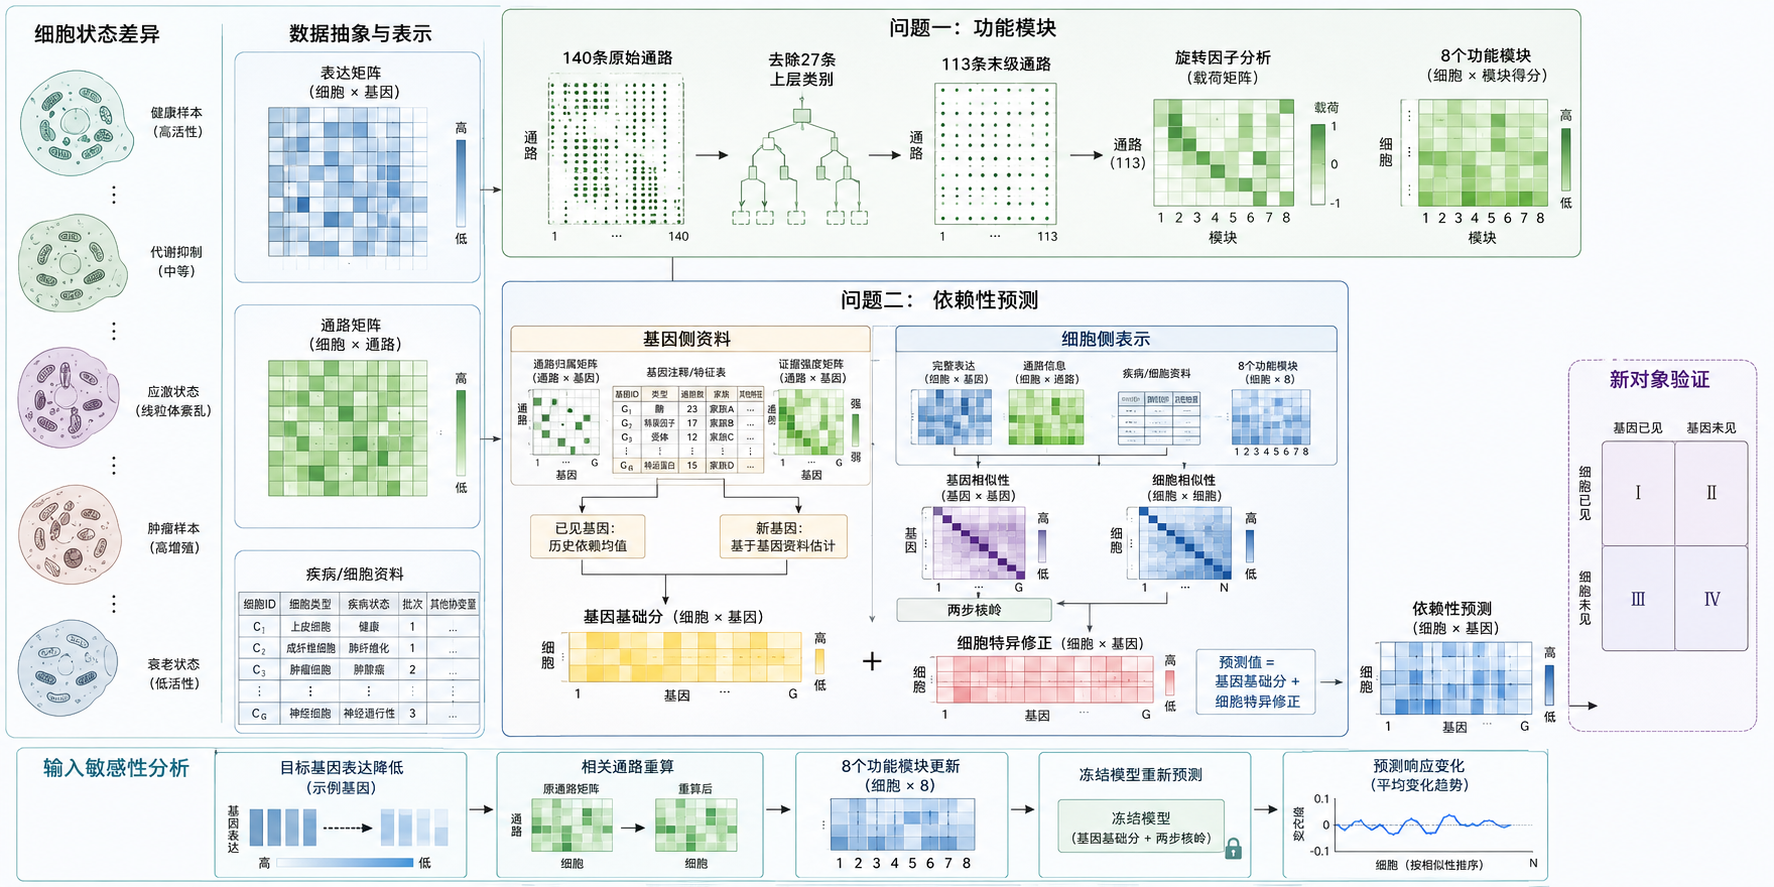
\includegraphics[width=\linewidth]{figures/OURWORK.png}
  \caption{本文总体研究路线\protect\cite{ref20}}
  \label{fig:overview}
\end{figure}

\hypertarget{21-ux6570ux636eux7ed3ux6784ux63edux793aux7684ux6838ux5fc3ux56f0ux96be}{%
\subsection{2.1 数据结构揭示的核心困难}\label{21-ux6570ux636eux7ed3ux6784ux63edux793aux7684ux6838ux5fc3ux56f0ux96be}}

训练表中的一行只记录一个细胞---基因组合，细胞状态和基因属性则分别存放在不同数据表中。数据整理时先按细胞标识连接表达、通路和疾病资料，再按基因名称连接基因注释。训练标签共有 872643 条，覆盖 1019 个细胞和 933 个基因；正式测试覆盖 1140 个细胞和 1098 个基因，其中包括 121 个新细胞、165 个新基因和 19858 个双侧新对象组合。

这使问题区别于普通矩阵补全。待预测位置不仅是矩阵中的空格，还可能来自训练数据从未出现过的整行或整列。若随机拆分标签，同一细胞和同一基因往往会同时出现在训练与验证中，所得成绩会高估新对象外推能力。为此，我们按照细胞和基因是否在训练中出现，将验证组合划分为旧细胞---旧基因、旧细胞---新基因、新细胞---旧基因和新细胞---新基因四类。

数学上，一个预测样本同时由细胞 \(c\) 和基因 \(g\) 决定：

\begin{equation}
\label{eq:pairwise-task}
\widehat y_{cg}=f(\boldsymbol x_c,\boldsymbol q_g),
\end{equation}

其中 \(\boldsymbol x_c\) 和 \(\boldsymbol q_g\) 分别表示细胞与基因资料。只有把两侧可迁移特征写入模型，才可能处理训练中没有历史标签的新对象。

四类新旧对象的组合结构将在图\ref{fig:cold-start-structure}中汇总。

\placeholderfigure{数据结构与四类冷启动图待重画}{数据结构与四类冷启动组合}{fig:cold-start-structure}

\hypertarget{22-ux4eceux901aux8defux8bfbux6570ux5230ux7ec6ux80deux529fux80fdux72b6ux6001}{%
\subsection{2.2 从通路读数到细胞功能状态}\label{22-ux4eceux901aux8defux8bfbux6570ux5230ux7ec6ux80deux529fux80fdux72b6ux6001}}

预测某个细胞依赖哪些基因之前，首先要回答``这是一个怎样的细胞''。题目给出的 140 条通路同时包含上层类别和末级功能，同一表达变化可能被上下级通路重复描述；通路间的相关性又使逐项解释十分困难。因此，问题一的目标并非单纯压缩变量数量，而是把层级重叠、共同变化的通路整理成少量可追溯的功能坐标。

实际处理先识别通路层级，仅让 113 条末级通路进入计算，上层类别保留用于模块命名。随后利用因子分析寻找驱动多条通路共同变化的潜在状态，并比较不同因子数。模块数量过少会混合多种功能，过多则产生支撑通路很少、难以解释的坐标，因此需要同时考虑信息覆盖和解释稳定性。主成分分析作为对照，用于判断单纯追求方差解释是否会把多类功能挤入同一方向。

\hypertarget{23-ux4eceux57faux56e0ux7684ux4e00ux822cux4f9dux8d56ux5230ux5177ux4f53ux7ec6ux80deux7684ux7279ux6b8aux4f9dux8d56}{%
\subsection{2.3 从基因的一般依赖到具体细胞的特殊依赖}\label{23-ux4eceux57faux56e0ux7684ux4e00ux822cux4f9dux8d56ux5230ux5177ux4f53ux7ec6ux80deux7684ux7279ux6b8aux4f9dux8d56}}

八个功能模块能够概括细胞状态，但仍未回答某个基因在该细胞中有多重要。训练标签显示，不同基因本身存在较稳定的总体差异：有些基因在许多细胞中都较重要，有些基因整体影响较弱。由此得到第一层估计，即先计算基因的一般依赖水平。

基础分仍会把同一基因在不同细胞中的预测压到相近位置。细胞的表达、通路和疾病背景可能使其对某个基因格外敏感，因而还需估计具体组合相对基础分的偏移。依赖性由此分解为

\begin{equation}
\label{eq:dependency-decomposition}
\widehat y_{cg}=b_g+\widehat r_{cg},
\end{equation}

其中 \(b_g\) 回答``这个基因通常有多重要''，\(r_{cg}\) 描述细胞背景使依赖性上升或下降了多少。对于没有历史标签的新组合，可利用相似细胞和相似基因的已观测偏移进行推断。于是，模型选择形成一条连续路线：岭回归补足新基因的基础分，两步核岭同时沿细胞和基因两侧传递特异修正，四类新对象验证则检验这套推断能否真正迁移。

\hypertarget{24-ux76f8ux5173ux7814ux7a76ux4e0eux5efaux6a21ux5207ux5165ux70b9}{%
\subsection{2.4 相关研究与建模切入点}\label{24-ux76f8ux5173ux7814ux7a76ux4e0eux5efaux6a21ux5207ux5165ux70b9}}

线粒体功能难以用单个指标概括。MitoCarta3.0 将线粒体蛋白按亚细胞位置和功能通路整理，为功能表示提供了较完整的先验体系\cite{ref4}；组学研究也常把高维基因或蛋白信息汇总到通路层面，以观察能量代谢、遗传信息维护和蛋白稳态等功能的协同变化\cite{ref6,ref7,ref8}。本题已有统一口径的通路得分，适合从这些读数中提取公共功能状态。

Cancer Dependency Map 和 Chronos 等工作表明，大规模 CRISPR 数据能够同时刻画共同必需基因和情境特异依赖\cite{ref2,ref3}。DeepDEP、BioVNN 与细胞特异网络模型进一步说明，多源组学、通路层级和网络信息可以支持未筛选对象的依赖性预测\cite{ref17,ref18,ref19}。这些研究共同提示：预测既要保留基因的总体规律，也要容纳细胞背景造成的差异。

岭回归能够形成有竞争力的依赖性预测基线\cite{ref9}，归纳矩阵补全和成对核岭回归则说明，两侧对象的自身特征可以支持新细胞或新基因的外推\cite{ref10,ref11,ref12}。据此，我们将``基因一般依赖''和``细胞特异偏移''分开处理，在固定四类验证中比较模型，避免仅凭结构复杂度作出选择。

\hypertarget{ux4e09ux6a21ux578bux5047ux8bbe}{%
\section{三、模型假设}\label{ux4e09ux6a21ux578bux5047ux8bbe}}

\begin{enumerate}
\def\labelenumi{\arabic{enumi}.}
\tightlist
\item
  题目给出的依赖性标签方向正确，在训练数据的统一测量口径下可以比较；标签越大表示细胞对相应基因的依赖越强。
\item
  基因表达和通路得分能够表征细胞之间的相对线粒体状态，但不直接对应蛋白活性、代谢通量或 ATP 产量。
\item
  上下级通路共享大量基因。为避免同一表达信号被重复放大，仅使用末级通路建立功能模块。
\item
  模块载荷表示通路在当前样本中的共同变化关系，不据此推断因果调控。
\item
  新细胞和新基因的标签在相应训练折中完全不可见；标准化、调参和路线选择均在训练数据内部完成。
\item
  同一细胞中的多条标签共享细胞背景，统计比较以细胞为配对单位。
\end{enumerate}

\hypertarget{ux56dbux7b26ux53f7ux8bf4ux660eux4e0eux6570ux636eux8868ux793a}{%
\section{四、符号说明与数据表示}\label{ux56dbux7b26ux53f7ux8bf4ux660eux4e0eux6570ux636eux8868ux793a}}

\hypertarget{41-ux4e3bux8981ux7b26ux53f7}{%
\subsection{4.1 主要符号}\label{41-ux4e3bux8981ux7b26ux53f7}}

主要符号及含义见表\ref{tab:symbols}。

\begin{longtable}[]{@{}ll@{}}
\caption{主要符号说明}\\
\toprule
符号 & 含义 \\
\midrule
\endhead
\(c\) & 细胞系索引 \\
\(g\) & 扰动基因索引 \\
\(p\) & 末级功能通路索引 \\
\(k\) & 功能模块索引 \\
\(y_{cg}\) & 细胞\(c\) 对基因 \(g\) 的真实依赖性标签 \\
\(\widehat y_{cg}\) & 模型预测的依赖性分数 \\
\(\boldsymbol x_c\) & 细胞侧特征向量 \\
\(\boldsymbol q_g\) & 基因侧特征向量 \\
\(\boldsymbol X\) & 标准化后的细胞---末级通路矩阵 \\
\(\boldsymbol Z\) & 细胞---模块得分矩阵 \\
\(\boldsymbol\Lambda\) & 通路---模块载荷矩阵 \\
\(b_g\) & 基因基础依赖性分数 \\
\(r_{cg}\) & 细胞---基因特异修正量 \\
\bottomrule
\end{longtable}
\label{tab:symbols}

\hypertarget{42-ux6570ux636eux8868ux53caux7528ux9014}{%
\subsection{4.2 数据表及用途}\label{42-ux6570ux636eux8868ux53caux7528ux9014}}

各数据表在建模中的用途见表\ref{tab:data-sources}。

\begin{longtable}[]{@{}p{2.4cm}p{5.2cm}p{7.2cm}@{}}
\caption{数据表及主要用途}\\
\toprule
数据 & 主要内容 & 用途 \\
\midrule
\endhead
细胞表达矩阵 & 1140 个细胞系的线粒体相关基因表达 & 构建通路、细胞特征和局部表达扰动输入 \\
通路得分矩阵 & 1140 个细胞系、140 条线粒体通路 & 问题一的模块提取与问题二的细胞侧特征 \\
细胞元数据 & 组织谱系、原发疾病和亚型 & 补充细胞背景信息 \\
基因元数据 & 定位、通路、结构域、同源性、共表达和质谱证据 & 新基因基础分与基因侧相似性 \\
训练标签 & 872643 个细胞---基因组合 & 拟合和固定冷启动验证 \\
正式测试模板 & 373990 个待预测组合 & 生成最终提交结果 \\
\bottomrule
\end{longtable}
\label{tab:data-sources}

\hypertarget{ux4e94ux95eeux9898ux4e00ux7ebfux7c92ux4f53ux529fux80fdux6a21ux5757ux6784ux5efa}{%
\section{五、问题一：线粒体功能模块构建}\label{ux4e94ux95eeux9898ux4e00ux7ebfux7c92ux4f53ux529fux80fdux6a21ux5757ux6784ux5efa}}

\hypertarget{51-ux901aux8defux5c42ux7ea7ux6574ux7406}{%
\subsection{5.1 通路层级整理}\label{51-ux901aux8defux5c42ux7ea7ux6574ux7406}}

\hypertarget{511-ux5c42ux7ea7ux6574ux7406}{%
\subsubsection{5.1.1 层级整理}\label{511-ux5c42ux7ea7ux6574ux7406}}

原始矩阵中的 140 条通路并非同一层级。若上层类别与下级通路同时进入模型，同一批基因的变化可能被重复计算。我们依据通路描述识别叶节点，使上层类别只参与功能解释，最终保留 113 条末级通路作为因子分析输入。

层级整理后，通路间的数值重复明显减弱。全部通路的相关矩阵秩为 134，绝对相关系数不低于 0.95 的通路对有 25 对；末级通路矩阵恢复满秩，高相关通路对降至 3 对。该结果说明，层级筛选确实减少了由重复定义造成的共线性。

\hypertarget{512-ux56e0ux5b50ux5206ux6790ux9002ux7528ux6027}{%
\subsubsection{5.1.2 因子分析适用性}\label{512-ux56e0ux5b50ux5206ux6790ux9002ux7528ux6027}}

末级通路的 KMO 统计量为 0.963，说明不同通路之间存在较强的公共结构。Bartlett 球形检验得到

\[
\chi^2=189777.739,\qquad df=6328,\qquad p<0.001,
\]

可以拒绝``相关矩阵为单位阵''的假设。多条通路确有共同变化，将其归纳为少数公共模块具有统计依据。

\hypertarget{52-ux56e0ux5b50ux6570ux7684ux9009ux62e9}{%
\subsection{5.2 因子数的选择}\label{52-ux56e0ux5b50ux6570ux7684ux9009ux62e9}}

模块太少会把多种生物过程混在一起，太多则容易得到只有少数通路支撑、难以命名的坐标。为寻找两者之间的平衡，我们比较 8、12、15、18 个因子。共同度衡量公共模块对原通路变化的覆盖程度；强载荷模块数和类别集中度则反映模块是否具备稳定的解释基础。

候选因子数的比较结果见表\ref{tab:factor-counts}。

\begin{longtable}[]{@{}r>{\centering\arraybackslash}p{2.2cm}>{\centering\arraybackslash}p{3.4cm}>{\centering\arraybackslash}p{4.2cm}>{\centering\arraybackslash}p{3.1cm}@{}}
\caption{不同因子数方案的质量比较}\label{tab:factor-counts}\\
\toprule
因子数 & 平均共同度 & 共同度不低于 0.50 的通路数 & 至少含 3 条强载荷通路的模块数 & 前 8 通路平均类别集中度 \\
\midrule
\endhead
8 & 0.6762 & 95 & 7 & 0.7188 \\
12 & 0.7120 & 99 & 6 & 0.7188 \\
15 & 0.7324 & 102 & 8 & 0.6500 \\
18 & 0.7489 & 102 & 8 & 0.6875 \\
\bottomrule
\end{longtable}

因子数增加后，平均共同度继续提高，但解释难度同步上升。12 因子方案只有 6 个模块得到至少 3 条强载荷通路支撑；15 和 18 因子虽增加了覆盖，其余模块仍较零散，类别集中度也没有同步改善。八因子方案以较少坐标解释了平均 67.62\% 的通路变化，其中 7 个模块具备多条强载荷通路，在压缩程度和解释稳定性之间更均衡。

主成分分析提供了另一种压缩方式。前 18 个主成分累计解释 80.30\% 的变化，但第一主成分单独占 49.87\%，并对 108 条通路产生强载荷，更接近多类功能的整体升降。后续主成分又缺少足够的突出通路。由于问题一还要求解释每个功能坐标，最终选择八因子方案。

\hypertarget{53-ux6a21ux5757ux8f7dux8377ux5f97ux5206ux4e0eux65b9ux5411ux56faux5b9a}{%
\subsection{5.3 模块载荷、得分与方向固定}\label{53-ux6a21ux5757ux8f7dux8377ux5f97ux5206ux4e0eux65b9ux5411ux56faux5b9a}}

记标准化后的细胞---通路矩阵为 \(\boldsymbol X\in\mathbb R^{1140\times113}\)。因子模型把通路变化分为公共状态和通路特异部分：

\begin{equation}
\label{eq:factor-model}
\boldsymbol X=\boldsymbol Z\boldsymbol\Lambda^{\mathsf T}+\boldsymbol E,
\end{equation}

其中 \(\boldsymbol Z\) 为细胞模块得分，\(\boldsymbol\Lambda\) 为通路载荷。对细胞 \(c\) 的标准化通路向量 \(\boldsymbol x_c\)，Bartlett 得分为

\begin{equation}
\label{eq:bartlett-score}
\widehat{\boldsymbol z}_c=
\left(\boldsymbol\Lambda^{\mathsf T}\boldsymbol\Psi^{-1}\boldsymbol\Lambda\right)^{-1}
\boldsymbol\Lambda^{\mathsf T}\boldsymbol\Psi^{-1}\boldsymbol x_c,
\end{equation}

\(\boldsymbol\Psi\) 表示各通路的特异方差。该权重使特异噪声较大的通路对得分影响较小。

最大方差正交旋转使突出载荷尽量集中到少数组通路，便于识别每个坐标的主要含义。正交是统计表示中的解耦约束，并不意味着线粒体功能在生物学上相互独立。因子方向可以整体取反，为保持不同运行中的含义一致，将每个模块绝对载荷最大的通路固定为正方向。模块得分越高，表示细胞更接近正载荷通路所定义的状态；负载荷通路会向相反方向变化。

模块得分是基于 1140 个细胞系的标准化相对量，用于比较细胞间的功能配置，也可在载荷固定后描述同一细胞输入变化前后的相对移动。酶活性、代谢通量和 ATP 产量仍需额外实验测量。

\hypertarget{54-ux516bux4e2aux529fux80fdux6a21ux5757ux7684ux89e3ux91ca}{%
\subsection{5.4 八个功能模块的解释}\label{54-ux516bux4e2aux529fux80fdux6a21ux5757ux7684ux89e3ux91ca}}

八个模块的命名依据是旋转载荷最高的通路、通路上层类别和 MitoCarta3.0 的功能注释\cite{ref4}。M1 共有 72 条通路达到 \(|\lambda|\geq0.35\)，更像多类线粒体功能共同升降的宽方向，其最高载荷仍集中于遗传信息维护与表达；M2 至 M4 的主要含义较清楚。第 5 至第 7 模块的混合程度更高；第 8 模块只有 1 条通路达到该阈值，因此只作为探索性指标。

模块命名、强载荷数量和解释把握汇总于表\ref{tab:module-definitions}。

\begin{longtable}[]{@{}l p{3.2cm} r p{6.5cm} p{1.8cm}@{}}
\caption{八个功能模块的载荷依据与解释}\\
\toprule
模块 & 名称 & 强载荷数 & 主要高载荷通路及载荷 & 解释把握 \\
\midrule
\endhead
M1 & 线粒体综合状态与遗传信息表达 & 72 & mtDNA 复制 0.8941、mt-tRNA 修饰 0.8754、线粒体核糖体装配 0.8534 & 高 \\
M2 & 脂肪酸和支链氨基酸利用 & 37 & 脂肪酸氧化 0.6691、肉碱穿梭 0.6681、肉碱合成与转运 0.6612 & 高 \\
M3 & 解毒与氧化还原代谢 & 26 & 外源物代谢 0.7635、肟还原复合体 0.6692、硫代谢 0.6412 & 高 \\
M4 & 氧化磷酸化 & 24 & OXPHOS 亚基 0.8568、复合体 I 亚基 0.8526、复合体 IV 亚基 0.8298 & 高 \\
M5 & 复合体 II 与辅因子代谢 & 21 & 维生素 B12 代谢 0.6698、呼吸体装配 0.5882、复合体 II 亚基 0.5602 & 中 \\
M6 & 质量控制与铁稳态 & 7 & 铁稳态 0.4779、自噬 0.4587、硒蛋白 0.4358 & 中 \\
M7 & 维生素---血红素与能量缓冲 & 3 & 肌酸代谢 0.4466、维生素 A 代谢 0.4244、维生素 D 代谢 0.3707 & 中 \\
M8 & TCA---复合体 II 与动力学平衡 & 1 & TCA 循环 0.3531、细胞色素 0.3270、线粒体融合 0.3206 & 探索性 \\
\bottomrule
\end{longtable}
\label{tab:module-definitions}

通路载荷结构与模块解释质量见图\ref{fig:module-loadings}。

\begin{figure}[H]
  \centering
  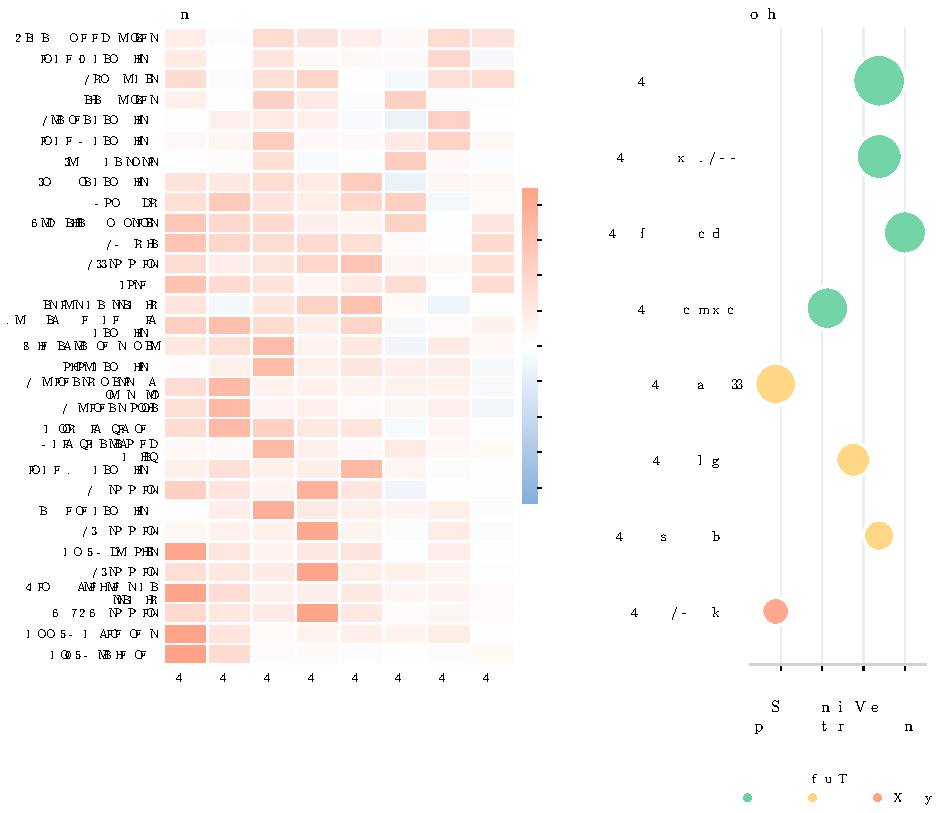
\includegraphics[width=\linewidth]{figures/result_q1_module_loadings_quality.pdf}
  \caption{通路载荷结构与八个功能模块的解释质量}
  \label{fig:module-loadings}
\end{figure}

M1 的强载荷覆盖代谢、蛋白导入、呼吸链和线粒体动力学等多类功能，其中最高载荷集中于 mtDNA 复制、核样体、mtRNA 加工和线粒体核糖体装配，因而命名为``线粒体综合状态与遗传信息表达''。M2 将脂肪酸氧化、肉碱转运和支链氨基酸代谢连在一起，反映脂质及部分氨基酸底物利用；M3 的核心通路涉及外源物代谢、硫代谢和谷胱甘肽相关反应；M4 则由多个呼吸链复合体亚基共同定义。

M5 跨越呼吸链与辅因子供应，M6 汇集质量控制和铁稳态，M7 主要涉及能量缓冲及辅因子代谢。这三个模块的功能混合程度高于 M2 至 M4。M8 的载荷较弱且来源分散，只作为补充观察坐标。

\hypertarget{55-ux95eeux9898ux4e00ux7ed3ux679c}{%
\subsection{5.5 问题一结果}\label{55-ux95eeux9898ux4e00ux7ed3ux679c}}

最终得到 \(1140\times8\) 的细胞模块得分矩阵和 \(113\times8\) 的通路载荷矩阵。八个坐标把高维通路状态整理成可解释的细胞功能表示，并保留了从模块回溯到原始通路的路径。

这里出现了从问题一走向问题二的关键区别：低维模块适合描述细胞，却未必保留依赖性预测所需的全部差异。若只用八个坐标进行预测，大量表达和通路细节会被压缩。因此，后续模型保留完整的表达、通路和疾病资料，把八模块作为具有解释意义的补充特征。功能模块负责回答``这是一个怎样的细胞''，完整资料则帮助判断该细胞会对哪些基因表现特殊。

不同组织谱系的模块状态见图\ref{fig:lineage-modules}。

\begin{figure}[H]
  \centering
  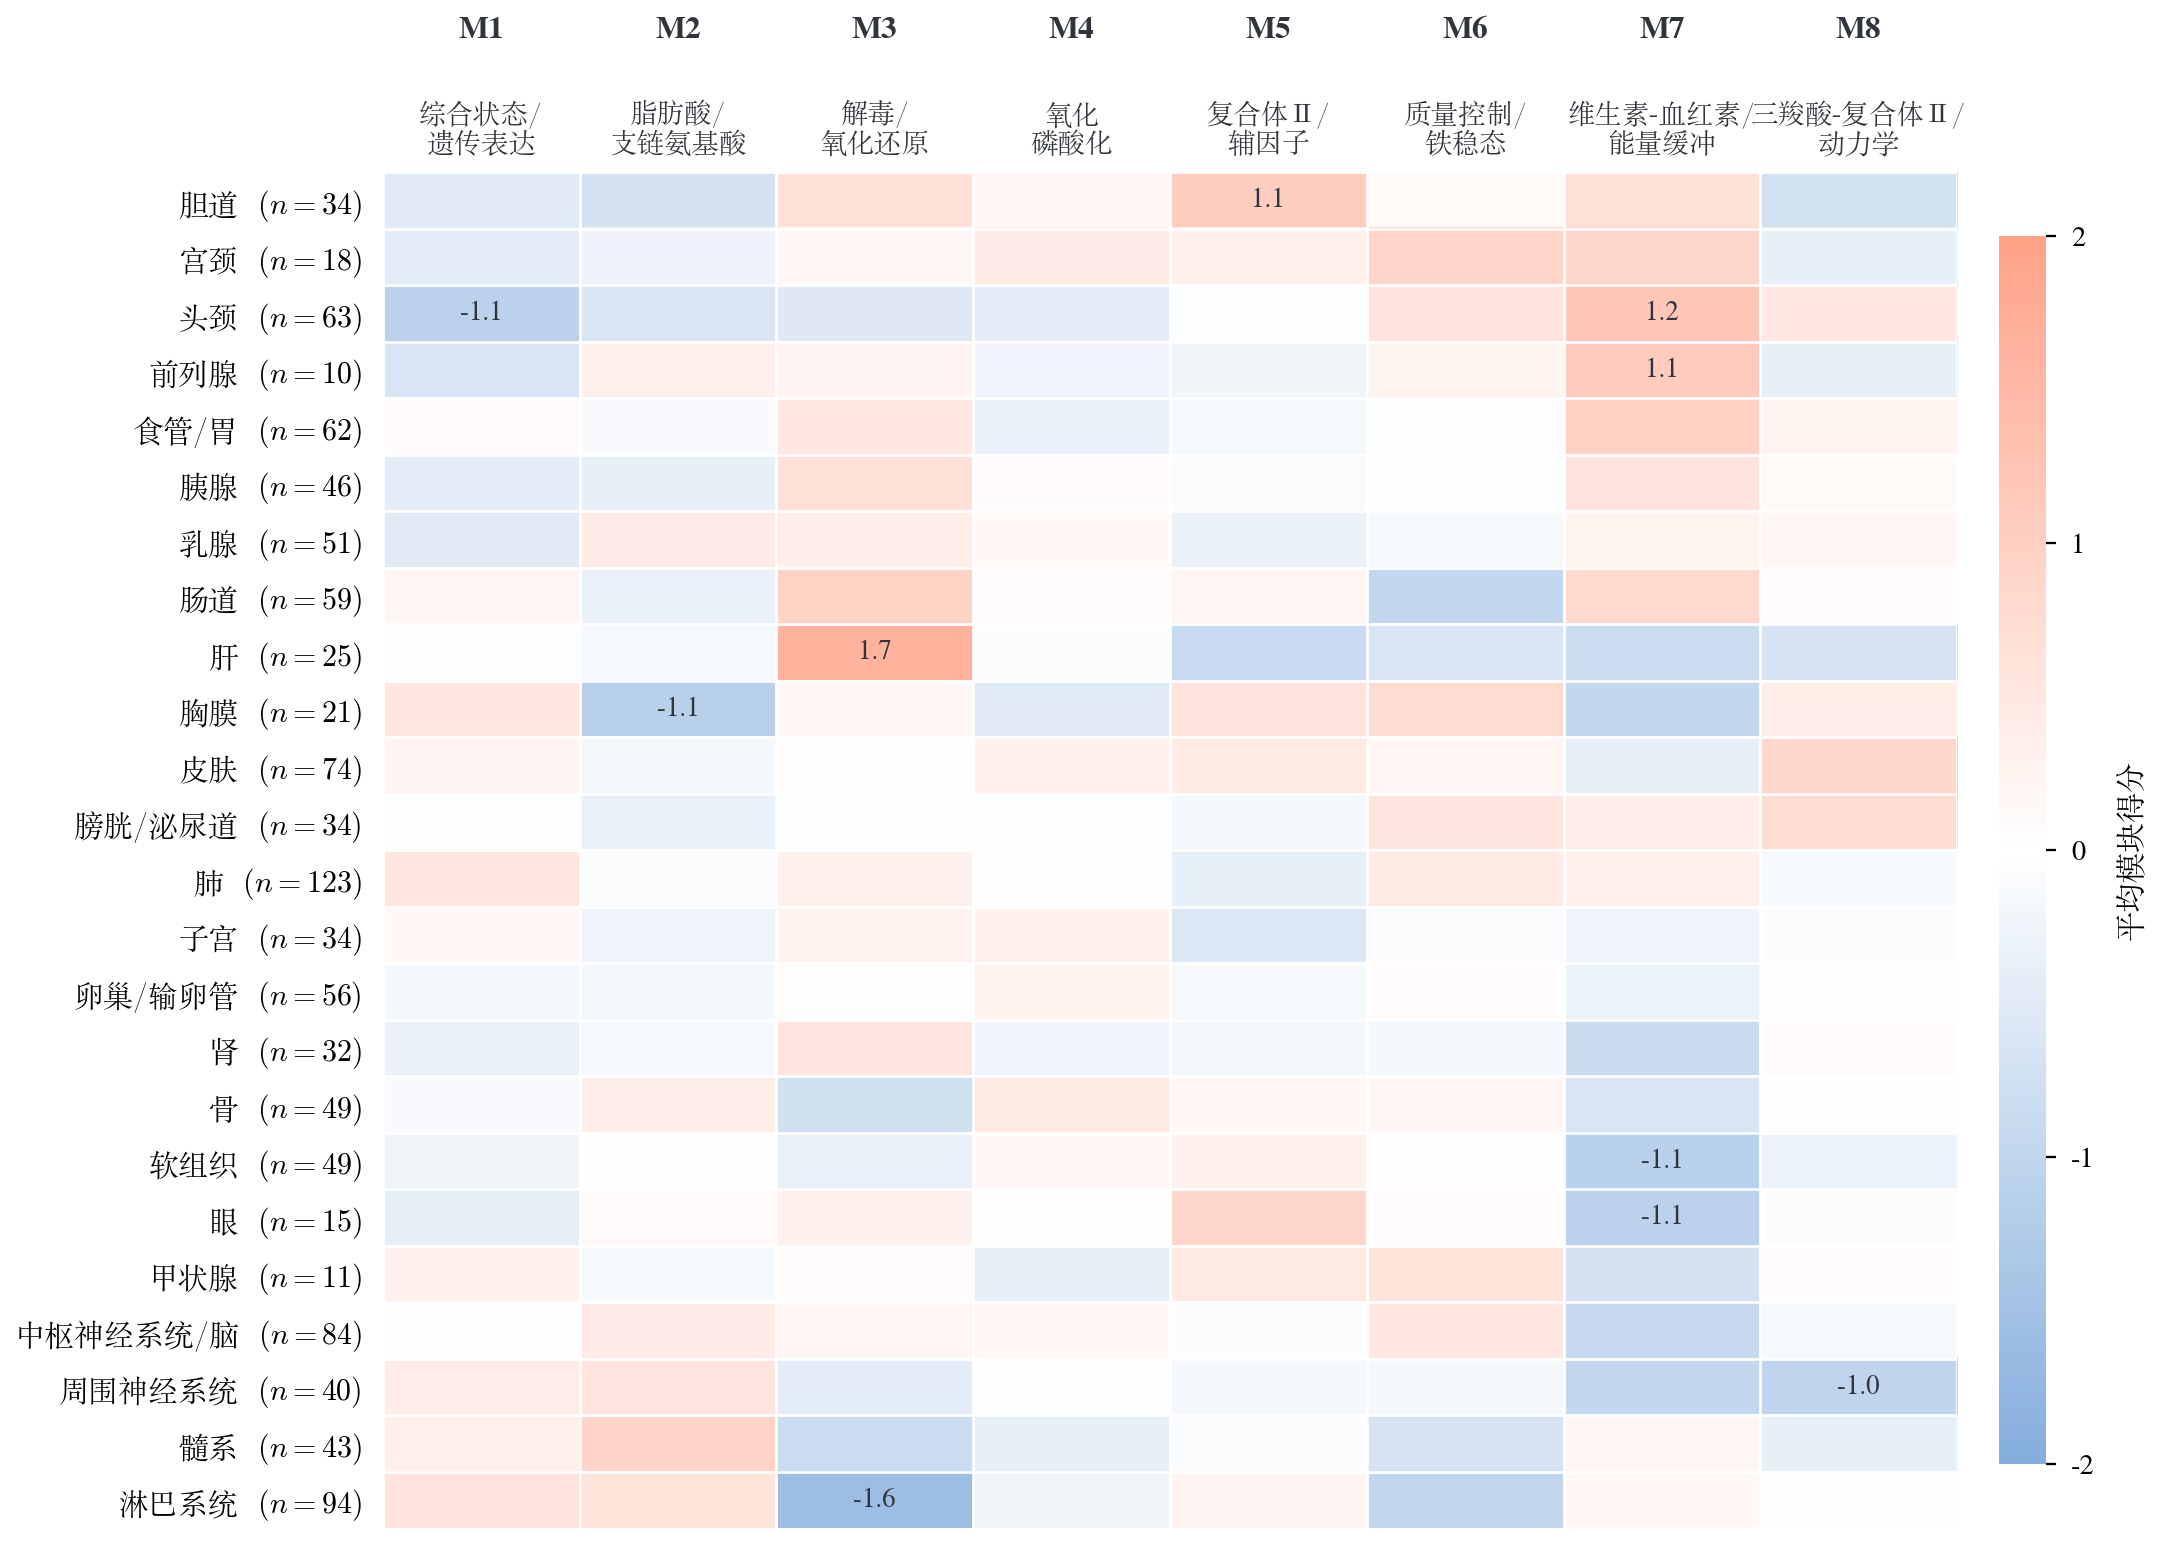
\includegraphics[width=0.86\linewidth]{figures/result_q1_lineage_module_state_preview.png}
  \caption{不同肿瘤组织谱系的八维功能模块状态}
  \label{fig:lineage-modules}
\end{figure}

\hypertarget{ux516dux95eeux9898ux4e8cux7ec6ux80deux57faux56e0ux4f9dux8d56ux6027ux9884ux6d4b}{%
\section{六、问题二：细胞---基因依赖性预测}\label{ux516dux95eeux9898ux4e8cux7ec6ux80deux57faux56e0ux4f9dux8d56ux6027ux9884ux6d4b}}

八模块说明了细胞的相对线粒体状态，但预测还要回答两个更具体的问题：一个基因通常有多重要，以及当前细胞为何会偏离这一一般水平。下面依次建立基因基础分和细胞特异修正，再用新对象验证检查模型能否迁移。

\hypertarget{61-ux65b0ux5bf9ux8c61ux9a8cux8bc1ux4e0eux53ccux4fa7ux7279ux5f81}{%
\subsection{6.1 新对象验证与双侧特征}\label{61-ux65b0ux5bf9ux8c61ux9a8cux8bc1ux4e0eux53ccux4fa7ux7279ux5f81}}

\hypertarget{611-ux6570ux636eux7ec4ux7ec7ux4e0eux9a8cux8bc1ux8bbeux8ba1}{%
\subsubsection{6.1.1 数据组织与验证设计}\label{611-ux6570ux636eux7ec4ux7ec7ux4e0eux9a8cux8bc1ux8bbeux8ba1}}

随机拆分会使同一细胞和同一基因同时出现在训练与验证中，从而低估新对象预测的难度。固定外层验证因此按对象划分，分别考察普通未测组合、仅细胞为新对象、仅基因为新对象以及双侧均为新对象四种情况；外层训练数据内部另设三组同类划分，用于选择模型和参数。

细胞侧使用基因表达、通路状态、疾病类型和八个功能模块，基因侧使用数值证据、功能类别、通路归属、证据词条和跨细胞表达轮廓。各类资料分别填补和标准化，并按维数调整尺度，避免高维表达块仅因列数较多而主导对象距离。验证时可以使用题目预先给出的对象侧资料，依赖性标签则始终与验证对象隔离。

\hypertarget{612-ux6570ux5b66ux8868ux793a}{%
\subsubsection{6.1.2 数学表示}\label{612-ux6570ux5b66ux8868ux793a}}

记细胞侧第 \(j\) 个资料块为 \(\boldsymbol X_c^{(j)}\)，基因侧第 \(l\) 个资料块为 \(\boldsymbol Q_g^{(l)}\)。每一块使用训练数据的尺度参数完成标准化：

\begin{equation}
\label{eq:block-standardization}
\widetilde{\boldsymbol X}^{(j)}=
\frac{\boldsymbol X^{(j)}-\boldsymbol\mu_j}
{\boldsymbol s_j\sqrt{d_j}},
\end{equation}

其中 \(d_j\) 为该块列数。各块横向拼接后形成细胞和基因的特征表示，对象编号不参与预测。目标基因在当前细胞中的单个表达值只用于双线性岭回归对照，不进入最终两步核岭。

双侧特征块及其含义见表\ref{tab:feature-blocks}。

\begin{longtable}[]{@{}p{2.0cm}p{5.6cm}p{7.2cm}@{}}
\caption{细胞侧、基因侧与组合侧特征块}\label{tab:feature-blocks}\\
\toprule
对象侧 & 特征块 & 主要含义 \\
\midrule
\endhead
细胞 & 表达、通路、疾病类型、八模块 & 当前细胞的分子状态和背景 \\
基因 & 数值证据、类别、通路、证据词条 & 基因自身资料与功能归属 \\
基因 & 跨细胞表达轮廓 & 该基因在不同细胞中的相对表达模式 \\
组合 & 目标基因自身表达 & 仅用于双线性岭回归对照，不进入最终两步核岭回归 \\
\bottomrule
\end{longtable}

\hypertarget{62-ux7b2cux4e00ux5c42ux57faux56e0ux7684ux4e00ux822cux4f9dux8d56}{%
\subsection{6.2 第一层：基因的一般依赖}\label{62-ux7b2cux4e00ux5c42ux57faux56e0ux7684ux4e00ux822cux4f9dux8d56}}

\hypertarget{621-ux4eceux5386ux53f2ux5747ux503cux5230ux65b0ux57faux56e0ux4f30ux8ba1}{%
\subsubsection{6.2.1 从历史均值到新基因估计}\label{621-ux4eceux5386ux53f2ux5747ux503cux5230ux65b0ux57faux56e0ux4f30ux8ba1}}

训练标签显示，基因之间存在明显的总体差异。对已见基因，跨细胞平均依赖性提供了最直接的一般水平；对新基因，这一历史均值不存在，只能从亚线粒体定位、通路归属、靶向信号、结构域、同源性、共表达和质谱证据中寻找相近规律。

基因资料既有连续变量，也有类别和缺失信息。连续变量以训练基因中位数填补并附加缺失指示，类别变量展开为哑变量。许多注释彼此相关，因此新基因的基础分采用带正则化的岭回归估计，惩罚参数在训练基因内部确定。

\hypertarget{622-ux6df7ux5408ux5cadux56deux5f52}{%
\subsubsection{6.2.2 混合岭回归}\label{622-ux6df7ux5408ux5cadux56deux5f52}}

设训练基因 \(g\) 的平均依赖性为

\begin{equation}
\label{eq:gene-mean}
m_g=\frac{1}{n_g}\sum_{c:(c,g)\in\mathcal D_{\mathrm{tr}}}y_{cg},
\end{equation}

基因元数据向量为 \(\boldsymbol q_g\)。岭回归通过

\begin{equation}
\label{eq:ridge-objective}
\min_{\beta_0,\boldsymbol\beta}
\sum_{g\in\mathcal G_{\mathrm{tr}}}
\left(m_g-\beta_0-\boldsymbol q_g^{\mathsf T}\boldsymbol\beta\right)^2
+\lambda_b\lVert\boldsymbol\beta\rVert_2^2
\end{equation}

学习新基因的基础分。最终采用混合规则：

\begin{equation}
\label{eq:mixed-base-score}
b_g=
\begin{cases}
m_g, & g\in\mathcal G_{\mathrm{tr}},\\
\beta_0+\boldsymbol q_g^{\mathsf T}\boldsymbol\beta,
& g\notin\mathcal G_{\mathrm{tr}}.
\end{cases}
\end{equation}

混合规则让旧基因保留更直接的实验均值，只在缺少标签时调用元数据回归。岭回归在依赖性预测中可以形成有竞争力的基线\cite{ref9}，并使基因总体差异与后续细胞修正保持清楚分工。

基因均值基线的外层总分为 53.08，引入新基因元数据后提高到 54.68；两个新基因组的 RMSE 分别由 0.372、0.375 降至 0.356、0.358。基因资料补足了部分历史信息，但基础分仍会让同一基因在不同细胞中的预测过于相似。这一不足引出了第二层模型。

不同基础分模型的结果比较见图\ref{fig:base-models}。

\begin{figure}[H]
  \centering
  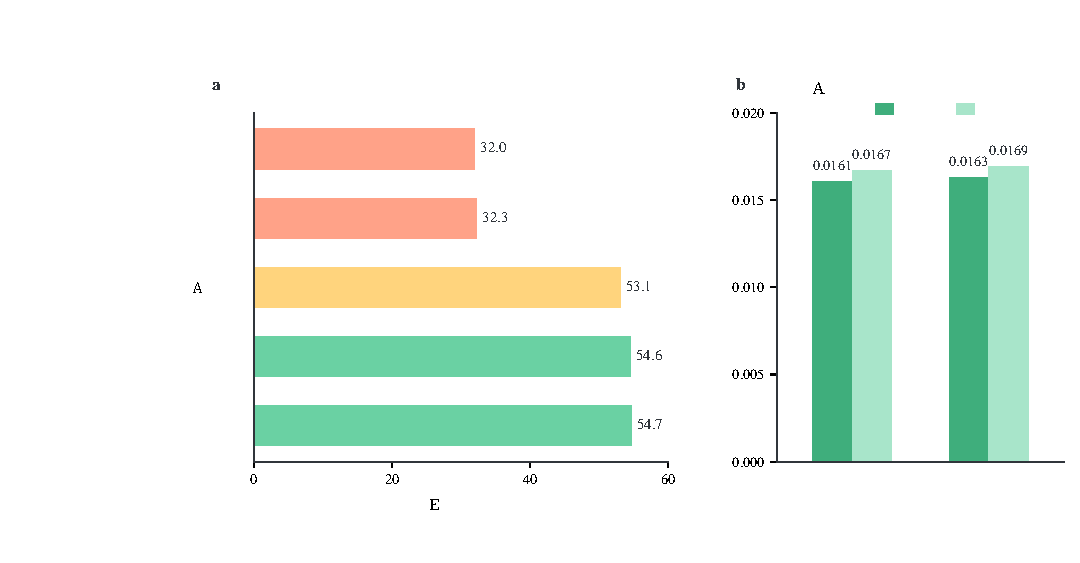
\includegraphics[width=0.90\linewidth]{figures/result_q2_gene_base_model_comparison.pdf}
  \caption{基因基础分模型的综合表现与新基因误差改善}
  \label{fig:base-models}
\end{figure}

\hypertarget{63-ux7b2cux4e8cux5c42ux7ec6ux80deux80ccux666fux9020ux6210ux7684ux7279ux5f02ux4feeux6b63}{%
\subsection{6.3 第二层：细胞背景造成的特异修正}\label{63-ux7b2cux4e8cux5c42ux7ec6ux80deux80ccux666fux9020ux6210ux7684ux7279ux5f02ux4feeux6b63}}

\hypertarget{631-ux6b8bux5deeux7684ux5b9eux9645ux542bux4e49}{%
\subsubsection{6.3.1 残差的实际含义}\label{631-ux6b8bux5deeux7684ux5b9eux9645ux542bux4e49}}

基因基础分已经回答``通常有多重要''，却无法解释同一个基因为何在不同细胞中表现不同。为把细胞背景单独提取出来，定义训练标签与基础分之差

\begin{equation}
\label{eq:residual}
e_{cg}=y_{cg}-b_g.
\end{equation}

残差为正，表示当前细胞对该基因的依赖高于一般水平；残差为负，则表示该细胞对它相对不敏感。\(e_{cg}\) 因而成为细胞背景造成的特异偏移。

对于没有测量过的组合，残差只能从已观测组合中借取。状态相近的细胞可能对同一基因产生相近偏移，功能相近的基因也可能在同一细胞背景下呈现相似变化。因此，我们分别构造细胞相似度和基因相似度，把已知残差沿两侧传递到新组合。两步核岭正适合这种由两类对象共同决定的预测任务\cite{ref10,ref11,ref12}。

\hypertarget{632-ux6838ux76f8ux4f3cux5ea6}{%
\subsubsection{6.3.2 核相似度}\label{632-ux6838ux76f8ux4f3cux5ea6}}

对任意两对象的平衡后特征 \(\boldsymbol u_i,\boldsymbol u_j\)，使用径向基核

\begin{equation}
\label{eq:rbf-kernel}
K_{ij}=\exp\left(-\frac{\lVert\boldsymbol u_i-\boldsymbol u_j\rVert_2^2}{2h}\right),
\end{equation}

其中 \(h\) 取训练对象两两正平方距离的中位数。由此得到细胞核 \(\boldsymbol K_c\) 和基因核 \(\boldsymbol K_g\)；核值越大，两个对象在现有资料中的整体状态越接近。

\hypertarget{633-ux4e24ux6b65ux4f20ux9012ux516cux5f0f}{%
\subsubsection{6.3.3 两步传递公式}\label{633-ux4e24ux6b65ux4f20ux9012ux516cux5f0f}}

将训练残差整理成细胞乘基因的矩阵 \(\boldsymbol R\)。固定外层训练矩形有 15.53\% 的位置未观测，故以``细胞平均偏移＋基因平均偏移－总体平均偏移''的加性模型补齐，暂不引入额外的组合交互。该值是矩阵求解所需的平滑初值，并非实验观测。记训练细胞和训练基因的核子矩阵为 \(\boldsymbol K_c^{\mathrm{tr}}\) 和 \(\boldsymbol K_g^{\mathrm{tr}}\)，则

\[
\boldsymbol A_c=\boldsymbol K_c(:,\mathcal C_{\mathrm{tr}})
\left(\boldsymbol K_c^{\mathrm{tr}}+\lambda\boldsymbol I\right)^{-1},
\]

\[
\boldsymbol A_g=\boldsymbol K_g(:,\mathcal G_{\mathrm{tr}})
\left(\boldsymbol K_g^{\mathrm{tr}}+\lambda\boldsymbol I\right)^{-1}.
\]

预测残差矩阵为

\begin{equation}
\label{eq:two-step-residual}
\widehat{\boldsymbol R}=\boldsymbol A_c\boldsymbol R\boldsymbol A_g^{\mathsf T},
\end{equation}

最终预测为

\begin{equation}
\label{eq:final-prediction}
\widehat y_{cg}=b_g+\widehat r_{cg}.
\end{equation}

第一步沿细胞相似性传递偏移，第二步沿基因相似性继续外推。细胞和基因同时为新对象时，两侧都依靠自身资料找到可借鉴的训练对象。

\hypertarget{634-ux4eceux7ebfux6027ux4ea4ux4e92ux5230ux76f8ux4f3cux6027ux4f20ux64ad}{%
\subsubsection{6.3.4 从线性交互到相似性传播}\label{634-ux4eceux7ebfux6027ux4ea4ux4e92ux5230ux76f8ux4f3cux6027ux4f20ux64ad}}

双线性岭回归先作为较简单的对照，它假设细胞特征与基因特征之间存在统一的线性交互。高维表达、通路和功能注释之间更可能呈现局部相似结构，因此进一步比较两步核岭。两种假设在三个内层划分中的最佳结果如下。

\begin{longtable}[]{@{}p{2.3cm}p{4.8cm}p{2.2cm}p{2.5cm}p{2.0cm}@{}}
\caption{双线性岭回归与两步核岭的内层比较}\label{tab:interaction-models}\\
\toprule
模型 & 对组合差异的假设 & 最佳参数 & 内层平均分变化 & 改善划分数 \\
\midrule
\endhead
双线性岭回归 & 两侧特征形成统一线性交互 & 0.001 & +0.135 & 2/3 \\
两步核岭 & 相似细胞和相似基因共享偏移模式 & 0.1 & \textbf{+0.420} & \textbf{3/3} \\
\bottomrule
\end{longtable}

两步核岭在三个划分中均超过基础分，说明直接利用两侧相似结构更适合当前数据，因而进入固定外层比较。

两步核岭的计算结构见图\ref{fig:two-step-structure}。

\begin{figure}[H]
  \centering
  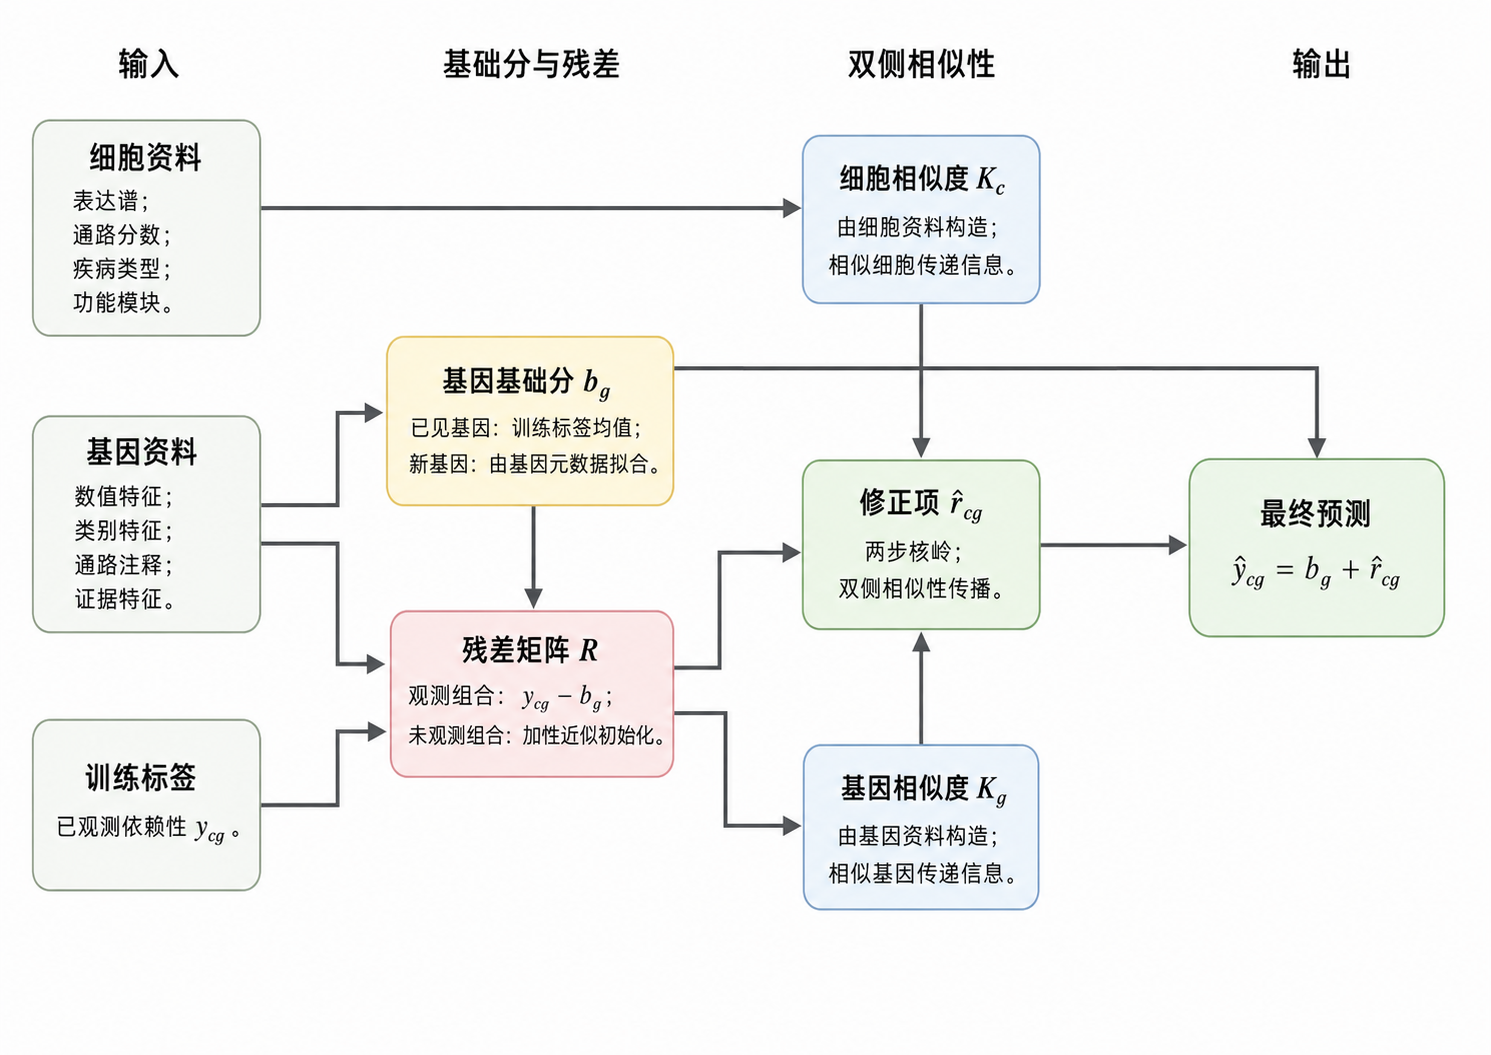
\includegraphics[width=\linewidth]{figures/result_q2_model_structure_revised.png}
  \caption{基因基础分与双侧相似性修正的两步核岭结构}
  \label{fig:two-step-structure}
\end{figure}

\hypertarget{64-ux5916ux5c42ux7ed3ux679cux4e0eux51b7ux542fux52a8ux8868ux73b0}{%
\subsection{6.4 外层结果与冷启动表现}\label{64-ux5916ux5c42ux7ed3ux679cux4e0eux51b7ux542fux52a8ux8868ux73b0}}

固定外层的总体指标见表\ref{tab:outer-metrics}。

\begin{longtable}[]{@{}lrrrrr@{}}
\caption{基础分模型与两步核岭的固定外层指标}\label{tab:outer-metrics}\\
\toprule
模型 & 总分 & \(\rho_{macro}\) & nDCG & Precision & RMSE \\
\midrule
\endhead
混合岭基础分 & 54.68 & \textbf{0.536} & 0.478 & 0.346 & 0.294 \\
两步核岭 & \textbf{55.29} & 0.533 & \textbf{0.485} & \textbf{0.359} & \textbf{0.285} \\
\bottomrule
\end{longtable}

两步核岭使总分提高 0.61，RMSE 相对下降约 3.22\%，nDCG 和 Precision 也有所提高。宏平均 Spearman 相关系数下降约 0.003。该模型能更准确地估计依赖值并识别前列候选，对完整基因序列的精细排序则略有退化。

四类冷启动结果如下。

\begin{longtable}[]{@{}lrrr@{}}
\caption{四类新旧对象组合的综合评分}\label{tab:cold-start-scores}\\
\toprule
组合类型 & 混合岭基础分 & 两步核岭 & 总分变化 \\
\midrule
\endhead
旧细胞---旧基因 & 79.41 & 80.30 & +0.89 \\
旧细胞---新基因 & 32.00 & 33.51 & \textbf{+1.51} \\
新细胞---旧基因 & 79.90 & 80.34 & +0.44 \\
新细胞---新基因 & 32.05 & 33.00 & \textbf{+0.95} \\
\bottomrule
\end{longtable}

四组均有提高，两个涉及新基因的组改善更明显，提示基因侧相似性补充了元数据基础分遗漏的部分信息。但新基因组的绝对得分仍约为 33，明显低于旧基因组的约 80，表明当前基因侧特征和外推方法仍不足以恢复其依赖模式。

四类组合的绝对得分及提升量见图\ref{fig:cold-start-scores}。

\begin{figure}[H]
  \centering
  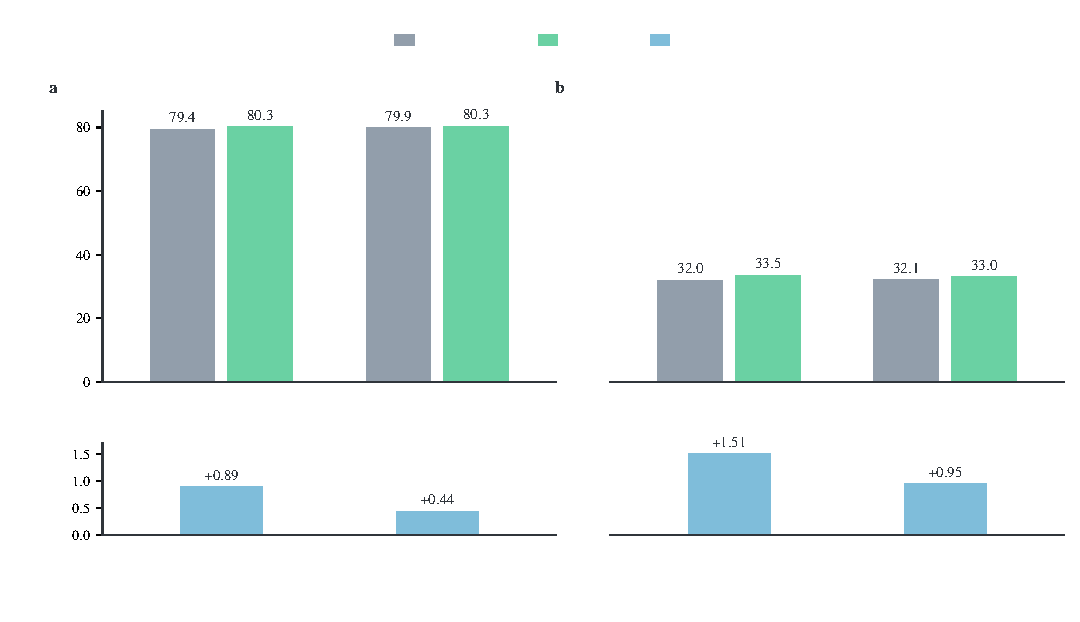
\includegraphics[width=0.86\linewidth]{figures/result_q2_cold_start_scores.pdf}
  \caption{两步核岭在四类冷启动组合中的综合评分}
  \label{fig:cold-start-scores}
\end{figure}

\hypertarget{65-ux5bf9ux7167ux6a21ux578bux4e0eux53d6ux820d}{%
\subsection{6.5 对照模型与取舍}\label{65-ux5bf9ux7167ux6a21ux578bux4e0eux53d6ux820d}}

两个关键对照进一步说明了最终模型为何同时保留低维模块、完整细胞资料和细胞内原始标签。

\begin{longtable}[]{@{}p{4.2cm}p{5.2cm}p{5.4cm}@{}}
\caption{影响最终模型结构的关键对照}\label{tab:model-ablation}\\
\toprule
对照思路 & 验证结果 & 得到的认识 \\
\midrule
\endhead
仅用低维模块和基因归属交互 & 最佳方案只比基础分高 0.02 & 可解释模块不足以代替完整细胞资料 \\
汇总不同细胞中的基因排名 & 总分降至 53.02，四项指标均下降 & 不同细胞内的名次缺少直接可比性 \\
\bottomrule
\end{longtable}

此外，按资料块赋权的多核在首个预筛划分中未显示增益，因而没有继续扩展；条件 RankRLS 虽使前列指标略升，却降低了新基因组和完整排序表现\cite{ref13,ref14}。最终由八模块承担状态解释，完整资料和细胞内原始标签承担预测。

\hypertarget{66-ux914dux5bf9ux7edfux8ba1ux68c0ux9a8c}{%
\subsection{6.6 配对统计检验}\label{66-ux914dux5bf9ux7edfux8ba1ux68c0ux9a8c}}

\hypertarget{661-ux4ee5ux7ec6ux80deux4e3aux914dux5bf9ux5355ux4f4d}{%
\subsubsection{6.6.1 以细胞为配对单位}\label{661-ux4ee5ux7ec6ux80deux4e3aux914dux5bf9ux5355ux4f4d}}

同一细胞中的多个基因共享细胞背景，逐行比较会高估独立样本数。因此，统计检验以细胞为配对单位：对 1019 个验证细胞进行 10000 次 Bootstrap 重采样，并在细胞内部完成配对置换。区间反映改善幅度在不同细胞中的稳定性，置换检验则判断观察到的提升能否由模型标签随机交换解释\cite{ref15}。

\hypertarget{662-ux68c0ux9a8cux7ed3ux679c}{%
\subsubsection{6.6.2 检验结果}\label{662-ux68c0ux9a8cux7ed3ux679c}}

各指标的观察变化与区间见表\ref{tab:paired-tests}。

\begin{longtable}[]{@{}lrr@{}}
\caption{两步核岭相对基础分模型的配对统计结果}\label{tab:paired-tests}\\
\toprule
指标 & 观察变化 & 95\% Bootstrap 区间 \\
\midrule
\endhead
官方总分 & +0.614 & {[}0.484, 0.746{]} \\
nDCG & +0.0067 & {[}0.0041, 0.0095{]} \\
Precision & +0.0133 & {[}0.0107, 0.0158{]} \\
RMSE 降低量 & +0.0095 & {[}0.0080, 0.0110{]} \\
\(\rho_{macro}\) & -0.0026 & {[}-0.0052, -0.0001{]} \\
\bottomrule
\end{longtable}

总分提升的单侧配对置换检验为 \(p=0.0001\)，置信区间也完全高于 0，说明综合改进在不同细胞中较为稳定。Spearman 的区间完全低于 0，证实完整排序的轻微下降同样具有一致性。综合得分提高的同时，完整排序略有下降，后续应用应侧重依赖值估计和前列候选识别。

各指标的配对变化分布见图\ref{fig:paired-improvement}。

\begin{figure}[H]
  \centering
  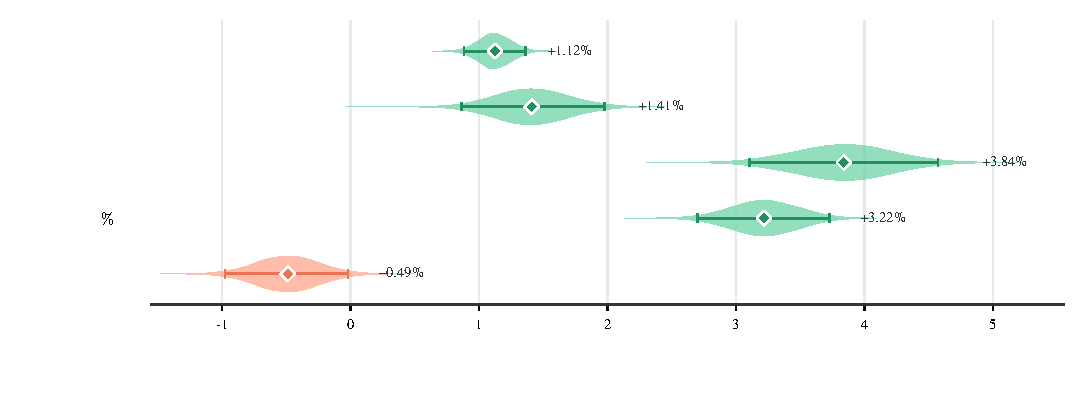
\includegraphics[width=0.88\linewidth]{figures/result_q2_paired_improvement.pdf}
  \caption{两步核岭相对基础分模型的配对指标变化}
  \label{fig:paired-improvement}
\end{figure}

\hypertarget{67-ux5c40ux90e8ux8868ux8fbeux6270ux52a8ux7684ux8f93ux5165ux654fux611fux6027}{%
\subsection{6.7 局部表达扰动的输入敏感性}\label{67-ux5c40ux90e8ux8868ux8fbeux6270ux52a8ux7684ux8f93ux5165ux654fux611fux6027}}

\hypertarget{671-ux5206ux6790ux76eeux7684ux4e0eux6270ux52a8ux8bbeux7f6e}{%
\subsubsection{6.7.1 分析目的与扰动设置}\label{671-ux5206ux6790ux76eeux7684ux4e0eux6270ux52a8ux8bbeux7f6e}}

为观察局部输入变化如何传递到通路、模块和依赖预测，从具有通路注释的高预测值组合中选取细胞和基因互不重复的 \texttt{HSPE1}、\texttt{PRELID1} 和 \texttt{ISCU} 三个案例。对目标基因的 \(\log(\mathrm{TPM}+1)\) 特征设置 50\%、75\% 和 100\% 三档扰动，分别表示从原表达状态向零表达状态移动相应比例的距离，其中 100\% 扰动对应表达完全关闭。

\hypertarget{672-ux8ba1ux7b97ux65b9ux6cd5}{%
\subsubsection{6.7.2 计算方法}\label{672-ux8ba1ux7b97ux65b9ux6cd5}}

设目标基因原表达的标准化值为 \(z_{cg}^{(0)}\)，零表达状态对应的标准化值为

\begin{equation}
\label{eq:zero-expression}
z_g^{(\mathrm{KO})}=\frac{0-\mu_g}{s_g+10^{-8}}.
\end{equation}

扰动强度 \(r\in[0,1]\) 时，在 \(\log(\mathrm{TPM}+1)\) 的标准化特征空间中线性插值

\begin{equation}
\label{eq:perturbation-path}
z_{cg}(r)=(1-r)z_{cg}^{(0)}+rz_g^{(\mathrm{KO})}.
\end{equation}

只重新计算包含目标基因的通路均值，再使用固定载荷和 Bartlett 规则更新八个模块，最后重新计算细胞核相似度和预测值；模型参数保持不变。

\hypertarget{673-ux6848ux4f8bux7ed3ux679c}{%
\subsubsection{6.7.3 案例结果}\label{673-ux6848ux4f8bux7ed3ux679c}}

三个敏感性案例的主要变化见表\ref{tab:sensitivity-cases}。

\begin{longtable}[]{@{}p{3.6cm}p{6.2cm}rr@{}}
\caption{局部表达扰动的三个案例结果}\label{tab:sensitivity-cases}\\
\toprule
细胞---基因 & 100\% 扰动时主要通路变化 & 最大模块变化 & 预测变化 \\
\midrule
\endhead
ACH-000618---HSPE1 & Chaperones -0.8688 & +0.2378 & -0.016912 \\
ACH-002677---PRELID1 & Cardiolipin synthesis -0.6757 & +0.4028 & +0.018028 \\
ACH-002475---ISCU & Fe-S cluster biosynthesis -0.4455 & -0.1571 & -0.001873 \\
\bottomrule
\end{longtable}

三个案例的通路变化范数和模块变化范数均随扰动强度单调增加，预测值也随之改变。两步核岭还综合了其余表达、疾病背景和基因资料，因此单个输入引起的预测变化小于中间通路和模块变化。已有研究也尝试从表达数据预测基因敲除效应\cite{ref16}；这里考察的是静态特征空间中的输入敏感性，不代表真实敲除后的因果效应。

三个案例的通路、模块与预测响应见图\ref{fig:counterfactual}。

\begin{figure}[H]
  \centering
  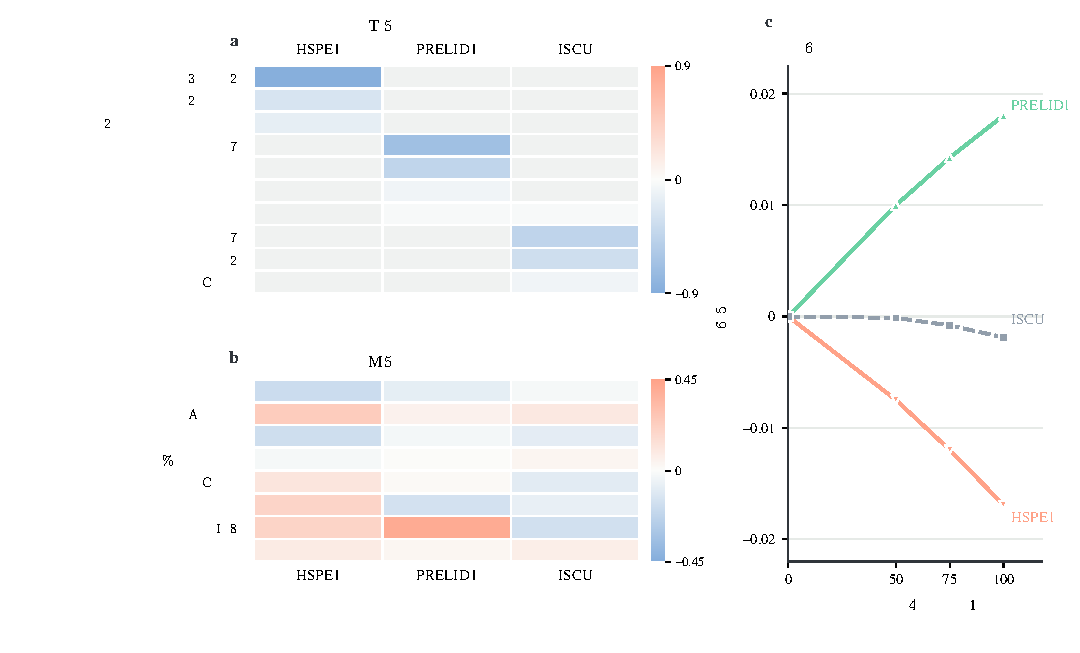
\includegraphics[width=0.98\linewidth]{figures/result_q2_counterfactual_chain.pdf}
  \caption{三个局部表达扰动案例的通路、模块与预测响应}
  \label{fig:counterfactual}
\end{figure}

\hypertarget{68-ux5168ux91cfux8badux7ec3ux4e0eux6b63ux5f0fux9884ux6d4b}{%
\subsection{6.8 全量训练与正式预测}\label{68-ux5168ux91cfux8badux7ec3ux4e0eux6b63ux5f0fux9884ux6d4b}}

模型结构和参数确定后，使用全部 872643 条训练标签重新拟合基因基础分和两步核岭。已见基因使用全量标签均值，新基因由元数据岭回归估计，残差模型保持验证阶段选定的参数。

全量模型生成 373990 个正式预测，覆盖 1140 个细胞和 1098 个基因。预测范围为 \([-0.456,3.892]\)，均值为 0.250，标准差为 0.290。测试标签尚不可见，这些数值用于提交和分布检查，真实预测效果以赛事评测为准。

四类新旧对象组合的正式预测分布见图\ref{fig:prediction-distribution}。旧基因两组的分布右尾更长，新基因两组则相对集中，反映出历史标签对基因基础分估计的影响。

\begin{figure}[H]
  \centering
  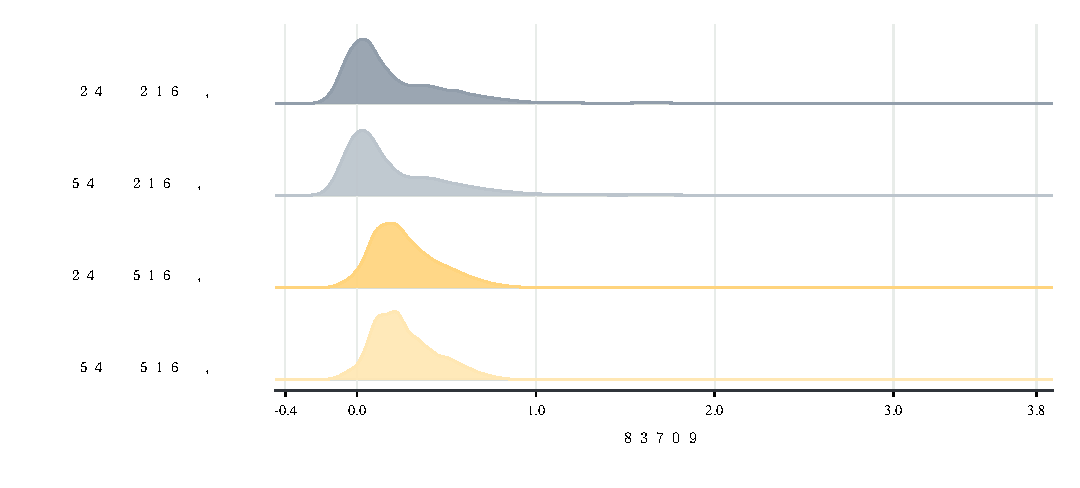
\includegraphics[width=0.98\linewidth]{figures/result_q2_prediction_distributions.pdf}
  \caption{四类新旧对象组合的正式预测分布（横轴显示 99.5\% 的预测值范围，少量右尾延伸至 3.892）}
  \label{fig:prediction-distribution}
\end{figure}

\hypertarget{ux4e03ux6a21ux578bux5206ux6790ux4e0eux68c0ux9a8c}{%
\section{七、模型分析与检验}\label{ux4e03ux6a21ux578bux5206ux6790ux4e0eux68c0ux9a8c}}

\hypertarget{71-ux65b0ux5bf9ux8c61ux9884ux6d4bux7684ux4e3bux8981ux56f0ux96be}{%
\subsection{7.1 新对象预测的主要困难}\label{71-ux65b0ux5bf9ux8c61ux9884ux6d4bux7684ux4e3bux8981ux56f0ux96be}}

四类外层验证结果呈现出一个明显差异：旧基因两组的综合得分均接近 80，而新基因两组仅为 33 左右；相比之下，同为旧基因或新基因时，新旧细胞之间的得分差距较小。这表明，当前模型的主要误差集中在基因侧，而不是细胞侧。

对于训练中已经出现的基因，可以利用大量历史标签估计其一般依赖水平。即使面对一个新细胞，这一基础信息仍然存在，再结合该细胞的表达、通路、疾病类型和功能模块，模型可以进一步估计细胞背景造成的偏移，因此新细胞---旧基因组仍取得了 80.34 的综合得分。

新基因则没有历史依赖标签，其基础分和细胞特异修正均需依靠功能注释、通路归属及相似基因进行外推。这些资料能够提供一定信息，但还不足以准确区分大量功能相近、依赖表现却不同的基因。双侧新对象组中，两步核岭使综合得分提高约 0.95，说明细胞与基因两侧的相似性确实能够补充部分缺失信息；但其绝对得分仍在 33 左右，也说明现有基因表征仍是预测链中最薄弱的一环。

因此，后续提升不应只依赖增加回归模型的复杂度。若输入资料仍不能充分区分新基因的功能和作用背景，更复杂的模型也可能只能重新组合已有信息，而难以弥补基因侧信息本身的不足。

\hypertarget{72-ux6570ux503cux8befux5deeux4e0eux6392ux5e8fux6307ux6807ux7684ux5deeux5f02}{%
\subsection{7.2 数值误差与排序指标的差异}\label{72-ux6570ux503cux8befux5deeux4e0eux6392ux5e8fux6307ux6807ux7684ux5deeux5f02}}

两步核岭加入细胞---基因特异修正后，RMSE、nDCG 和 Precision 均有所改善，但宏平均 Spearman 相关系数略有下降。几项指标的变化方向不同，与它们关注的对象不同有关。

模型使用平方误差拟合残差，预测偏差越大，训练中受到的惩罚越强。因此，它更容易优先修正依赖性较强、数值误差也较大的组合。高依赖基因的预测值和前列位置得到改善后，RMSE、nDCG 和 Precision 会随之提高。与此同时，大量位于排序中部、依赖性分数彼此接近的基因，可能因为细小的数值修正而发生前后换位。此类变化对前列筛选影响有限，却会降低基于完整序列计算的 Spearman 相关系数。

这一结果限定了模型的适用范围。当前模型更适合估计依赖性强度，并从每个细胞的大量候选基因中优先筛出少量高依赖对象；若应用目标是恢复全部基因的严格先后次序，则需要在数值误差之外进一步引入面向完整排序的约束，并重新检验这种调整是否会削弱新基因的外推表现。

图\ref{fig:phase7-application}概括了这一应用边界：模型首先结合细胞状态缩小候选基因范围，再将优先级较高的对象交由后续实验验证。

\begin{figure}[H]
  \centering
  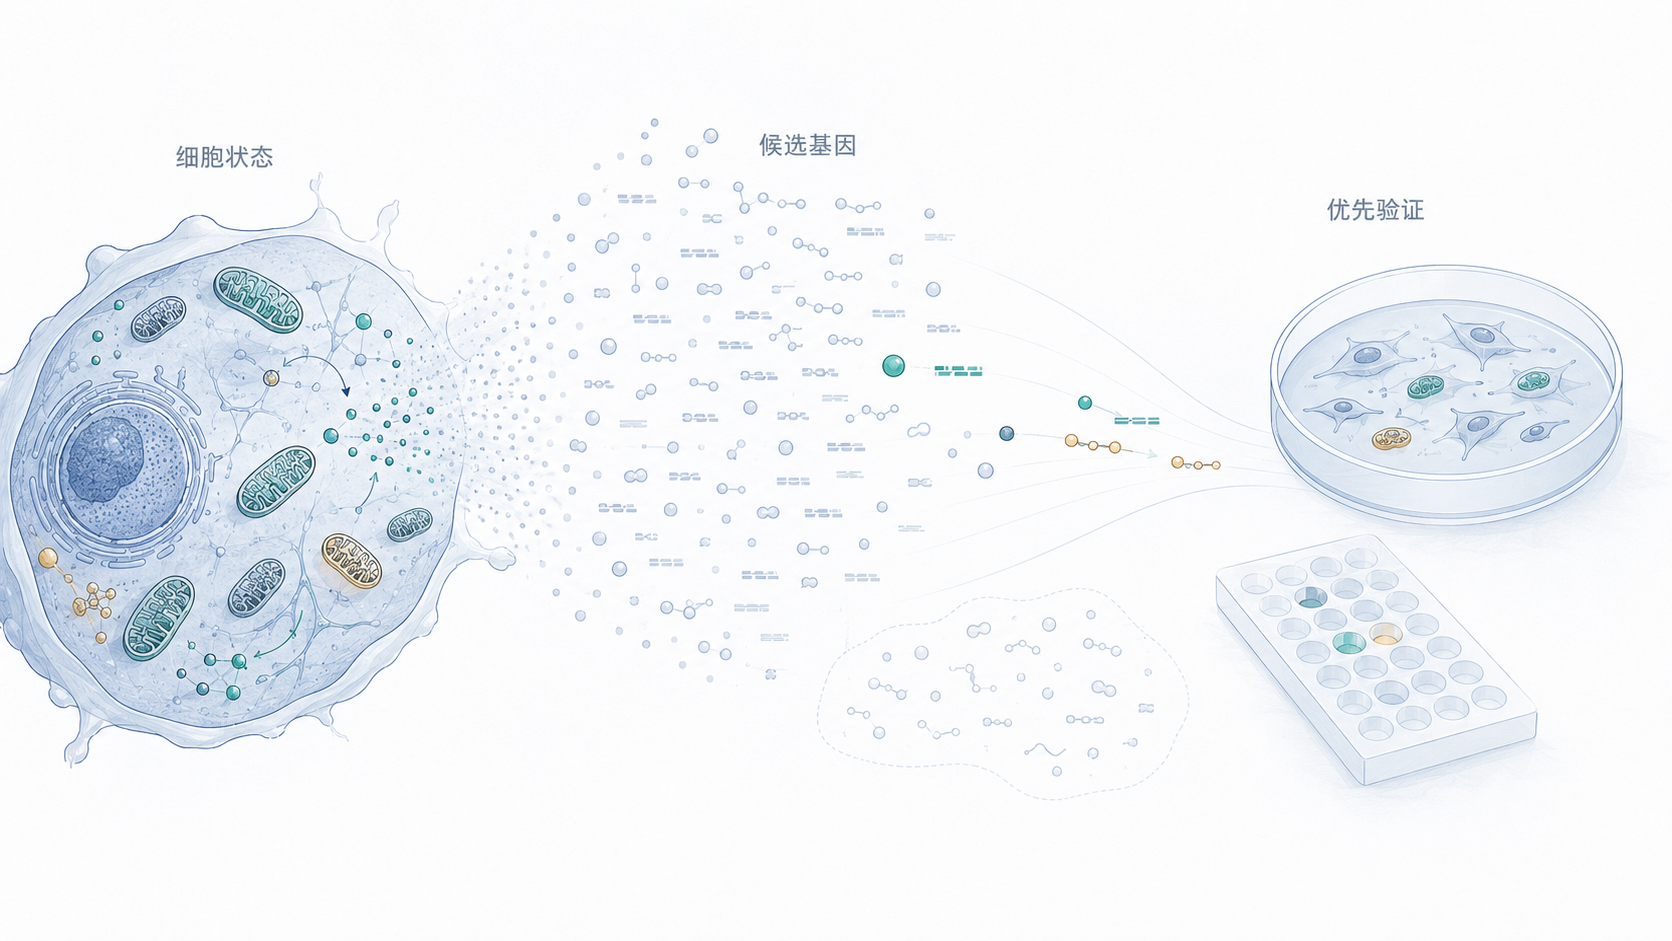
\includegraphics[width=\linewidth]{figures/addup-phase7.png}
  \caption{基于细胞状态的候选基因优先筛选流程\protect\cite{ref20}}
  \label{fig:phase7-application}
\end{figure}

\hypertarget{73-ux9a8cux8bc1ux8bbeux8ba1ux4e0eux7a33ux5b9aux6027ux68c0ux67e5}{%
\subsection{7.3 验证设计与稳定性检查}\label{73-ux9a8cux8bc1ux8bbeux8ba1ux4e0eux7a33ux5b9aux6027ux68c0ux67e5}}

模型选择和最终评价采用彼此分离的验证层次。三组内层冷启动划分用于比较候选模型和参数，固定外层验证集只在模型路线确定后使用一次，避免根据同一组外层结果反复调整方案。所有对象划分和随机过程均使用随机种子 42，以保证结果可以复现。

由于综合得分是由多个细胞的预测结果汇总而成，单一总分可能掩盖不同细胞之间的差异。为此，本文以细胞为配对单位进行 Bootstrap 和置换检验，考察总分改善是否只由少数细胞拉动。检验结果支持两步核岭相对于基础模型的综合增益，但对 Spearman 的小幅下降也应如实保留，不能仅根据总分提高判断所有指标均得到改善。

正式预测沿用验证阶段确定的数据处理、基因基础分和两侧相似性传播方法。训练和验证之间的依赖性标签保持隔离，题目预先提供的细胞与基因侧资料则按统一规则构造特征，从而使验证结果与最终模型保持相同的计算口径。

\hypertarget{ux516bux6a21ux578bux8bc4ux4ef7ux6539ux8fdbux4e0eux63a8ux5e7f}{%
\section{八、模型评价、改进与推广}\label{ux516bux6a21ux578bux8bc4ux4ef7ux6539ux8fdbux4e0eux63a8ux5e7f}}

\hypertarget{81-ux6a21ux578bux4f18ux70b9}{%
\subsection{8.1 模型优点}\label{81-ux6a21ux578bux4f18ux70b9}}

本文首先将依赖性拆分为基因的一般依赖水平和细胞背景造成的特异偏移。基因基础分吸收不同基因之间较稳定的整体差异，两步核岭则利用相似细胞和相似基因的已知结果，估计具体组合相对于基础分的上调或下调。与直接对所有标签进行统一回归相比，这一拆分使两类差异具有较清楚的含义，也便于分析误差究竟来自基因侧还是细胞侧。

验证方式针对正式测试中的新对象进行了设计。通过分别考察旧细胞---旧基因、旧细胞---新基因、新细胞---旧基因和新细胞---新基因，可以区分普通未测组合、单侧冷启动和双侧冷启动，而不会被随机拆分中重复出现的对象高估模型能力。内层选择和固定外层评价的分离，也减少了反复观察验证结果带来的选择偏差。

问题一得到的功能模块为细胞提供了较简洁的线粒体状态描述。最终预测没有只保留这八个模块，而是同时使用完整表达、通路和细胞资料，避免低维压缩丢失过多预测信息；模块则作为具有生物解释的补充特征，并用于观察局部表达变化如何传递到通路状态和预测结果。

\hypertarget{82-ux6a21ux578bux5c40ux9650}{%
\subsection{8.2 模型局限}\label{82-ux6a21ux578bux5c40ux9650}}

当前最明显的限制是新基因预测能力不足。旧基因可以从历史标签中获得较稳定的基础分，新基因只能依赖已有元数据和相似基因外推。虽然两步核岭提高了新基因两组的综合得分，但其绝对表现仍明显低于旧基因组，说明现有基因资料尚不足以完整刻画基因在不同细胞中的依赖差异。

训练标签没有覆盖所有训练细胞和训练基因的组合。本文以细胞平均残差和基因平均残差构造加性填充值，相当于先假定未观测位置不存在额外的组合特异作用，再由两侧相似性对其进行修正。这一处理使残差矩阵能够进入两步核岭计算，但可能平滑掉少数强烈的细胞---基因交互。现有验证支持包含该步骤的完整预测链，并不能单独证明这些填充值接近真实实验结果。

模型还使用了题目预先给出的全部对象侧资料，包括跨细胞表达轮廓。因此，本文评价的是已知测试对象特征条件下的传导式预测。如果实际应用中连未来细胞的表达和通路资料也无法提前获得，则需要采用更严格的纯归纳划分重新训练和评价。

八个功能模块来源于当前细胞集合中的统计共变结构，并不等同于八个彼此独立、已经得到实验确认的生物机制。前四个模块具有相对清楚的功能指向，后四个模块的解释仍需谨慎。局部表达扰动同样只发生在静态的 \(\log(\mathrm{TPM}+1)\) 特征空间，没有包含真实基因扰动后的补偿、反馈和时间变化，因此只能用于检查模型输入与输出之间的连续响应。

\hypertarget{83-ux6539ux8fdbux65b9ux5411}{%
\subsection{8.3 改进方向}\label{83-ux6539ux8fdbux65b9ux5411}}

后续工作的首要方向是补充新基因表征。现有通路归属和通用功能注释能够给出大致功能相似性，但对功能接近、依赖模式不同的基因区分能力有限。蛋白互作、复合物关系、亚细胞定位以及样本特异的调控网络，可能为新基因提供更具区分力的信息。新增资料仍应在相同的新基因和双侧冷启动划分中评价，避免因已见基因表现提高而掩盖真正的外推能力。

第二个方向是减少对残差矩阵填补的依赖。可以考虑直接在已观测细胞---基因索引上求解的成对核方法，使模型只利用真实标签估计交互结构，而不必先为所有缺失位置赋值。与此同时，可进一步比较兼顾平方误差、前列筛选和完整排序的联合目标，检验排序改善是否会以数值精度或新基因表现下降为代价。

若能够获得真实扰动后的时序表达、蛋白或代谢数据，则可以在扰动后重新计算通路与模块状态，并研究细胞的补偿和反馈过程。届时，当前的静态输入敏感性分析可以扩展为基于真实观测的动态响应模型，其结论也将更接近实际生物扰动过程。

\hypertarget{ux4e5dux7ed3ux8bba}{%
\section{九、结论}\label{ux4e5dux7ed3ux8bba}}

本题的预测难点并不只是补全未测量的细胞---基因组合，还包括对训练中从未出现的新细胞和新基因进行外推。为描述不同细胞的线粒体状态，本文先去除通路层级中的重复信息，再将 113 条末级通路归纳为八个功能模块。前四个模块具有相对清楚的功能指向，后四个模块则保留较谨慎的解释。该表示为 1140 个细胞提供了可由原始通路追溯的低维状态坐标，但预测时仍保留完整表达和通路资料，以避免过度压缩。

依赖性预测进一步区分了两类信息：基因基础分描述一个基因在一般细胞背景下的依赖水平，细胞---基因特异修正则描述具体细胞状态造成的偏移。两步核岭利用细胞和基因两侧的相似性估计这一偏移，使固定外层综合得分由 54.68 提高到 55.29，四类新旧对象组合均有改善。

指标变化表明，模型对依赖性数值和前列候选的判断有所提高，但并未全面改善完整基因序列的排序。因此，当前结果更适合用于缩小后续实验筛选范围，优先推荐少量可能具有较强依赖性的基因，而不宜被解释为所有候选基因的精确排序。

四类验证结果还显示，性能差距主要由基因是否具有历史标签决定。旧基因组的综合得分接近 80，新基因组仍只有 33 左右，说明新基因的功能表征是当前应用中的主要限制。模型已使用全部训练标签生成 373990 个正式预测；局部表达扰动结果则表明，输入变化能够沿通路、模块和预测过程传递，但这种静态响应尚不能替代真实扰动实验。进一步补充新基因的功能关系和扰动后观测，比单纯增加预测模型复杂度更值得优先研究\cite{ref21}。

\hypertarget{ux5341ux53c2ux8003ux6587ux732e}{%
\section{十、参考文献}\label{ux5341ux53c2ux8003ux6587ux732e}}

\bibliographystyle{gbt7714-numeric}
\bibliography{references}

% 以下为 Markdown 初稿中的人工参考文献清单，仅保留作迁移核对，不参与排版。
\iffalse

{[}1{]} GLOVER H L, SCHREINER A, DEWSON G, et al. Mitochondria and cell death{[}J{]}. Nature Cell Biology, 2024, 26(9): 1434-1446.

{[}2{]} ARAFEH R, SHIBUE T, DEMPSTER J M, et al. The present and future of the Cancer Dependency Map{[}J{]}. Nature Reviews Cancer, 2025, 25(1): 59-73.

{[}3{]} DEMPSTER J M, BOYLE I, VAZQUEZ F, et al. Chronos: a cell population dynamics model of CRISPR experiments that improves inference of gene fitness effects{[}J{]}. Genome Biology, 2021, 22(1): 343.

{[}4{]} RATH S, SHARMA R, GUPTA R, et al. MitoCarta3.0: an updated mitochondrial proteome now with sub-organelle localization and pathway annotations{[}J{]}. Nucleic Acids Research, 2021, 49(D1): D1541-D1547.

{[}5{]} GRANATH-PANELO M, KAJIMURA S. Mitochondrial heterogeneity and adaptations to cellular needs{[}J{]}. Nature Cell Biology, 2024, 26(5): 674-686.

{[}6{]} SCHÄFER J A, SUTANDY F X R, MÜNCH C. Omics-based approaches for the systematic profiling of mitochondrial biology{[}J{]}. Molecular Cell, 2023, 83(6): 911-926.

{[}7{]} TAN B G, GUSTAFSSON C M, FALKENBERG M. Mechanisms and regulation of human mitochondrial transcription{[}J{]}. Nature Reviews Molecular Cell Biology, 2024, 25(2): 119-132.

{[}8{]} BAKER Z N, FORNY P, PAGLIARINI D J. Mitochondrial proteome research: the road ahead{[}J{]}. Nature Reviews Molecular Cell Biology, 2024, 25(1): 65-82.

{[}9{]} CHANG D, ZHANG X. Ridge regression baseline model outperforms deep learning method for cancer genetic dependency prediction{[}EB/OL{]}. bioRxiv, 2023. DOI: 10.1101/2023.11.29.569083.

{[}10{]} STOCK M, PAHIKKALA T, AIROLA A, et al. A comparative study of pairwise learning methods based on kernel ridge regression{[}J{]}. Neural Computation, 2018, 30(8): 2245-2283.

{[}11{]} NATARAJAN N, DHILLON I S. Inductive matrix completion for predicting gene-disease associations{[}J{]}. Bioinformatics, 2014, 30(12): i60-i68.

{[}12{]} JAIN P, DHILLON I S. Provable inductive matrix completion{[}EB/OL{]}. arXiv:1306.0626, 2013.

{[}13{]} NASCIMENTO A C A, PRUDÊNCIO R B C, COSTA I G. A multiple kernel learning algorithm for drug-target interaction prediction{[}J{]}. BMC Bioinformatics, 2016, 17(1). DOI: 10.1186/s12859-016-0890-3.

{[}14{]} PAHIKKALA T, AIROLA A, STOCK M, et al. Efficient regularized least-squares algorithms for conditional ranking on relational data{[}J{]}. Machine Learning, 2013, 93(2-3): 321-356.

{[}15{]} GROSS B, DAUVIN A, CABELI V, et al. Robust evaluation of deep learning-based representation methods for survival and gene essentiality prediction on bulk RNA-seq data{[}J{]}. Scientific Reports, 2024, 14(1). DOI: 10.1038/s41598-024-67023-8.

{[}16{]} ROSENSKI J, SHIFMAN S, KAPLAN T. Predicting gene knockout effects from expression data{[}J{]}. BMC Medical Genomics, 2023, 16(1). DOI: 10.1186/s12920-023-01446-6.

{[}17{]} CHIU Y C, ZHENG S, WANG L J, et al. Predicting and characterizing a cancer dependency map of tumors with deep learning{[}J{]}. Science Advances, 2021, 7(34): eabh1275. DOI: 10.1126/sciadv.abh1275.

{[}18{]} LIN C H, LICHTARGE O. Using interpretable deep learning to model cancer dependencies{[}J{]}. Bioinformatics, 2021, 37(17): 2675-2681. DOI: 10.1093/bioinformatics/btab137.

{[}19{]} BENSTEAD-HUME G, WOOLLER S K, RENAUT J, et al. Biological network topology features predict gene dependencies in cancer cell-lines{[}J{]}. Bioinformatics Advances, 2022, 2(1): vbac084. DOI: 10.1093/bioadv/vbac084.
\fi

\hypertarget{ux5341ux4e00ux9644ux5f55}{%
\section{十一、附录}\label{ux5341ux4e00ux9644ux5f55}}

\hypertarget{ux9644ux5f55-a-ux652fux6491ux6570ux636eux8bf4ux660e}{%
\subsection{附录 A 支撑数据说明}\label{ux9644ux5f55-a-ux652fux6491ux6570ux636eux8bf4ux660e}}

随论文提交的支撑数据包含四类结果：1140 个细胞的八维模块得分及 113 条末级通路载荷；四类新旧对象组合的验证指标与配对统计结果；三个局部表达扰动案例的通路、模块和预测轨迹；373990 个待测组合的最终预测值。原始竞赛数据不重复附入论文。主要文件见表\ref{tab:appendix-data}。

\begin{longtable}[]{@{}p{6.2cm}p{8.6cm}@{}}
\caption{主要支撑数据文件}\label{tab:appendix-data}\\
\toprule
文件 & 内容 \\
\midrule
\endhead
\path{stage3_cell_module_scores.csv} & 1140 个细胞的八维模块得分 \\
\path{stage3_module_loadings.csv} & 113 条末级通路在八个模块上的载荷 \\
\path{stage7_official_metrics.csv} & 基础分与两步核岭的总体及四类冷启动指标 \\
\path{stage7_paired_test_summary.csv} & 按细胞配对的 Bootstrap 区间与置换检验结果 \\
\path{stage9_case_summary.csv}、\path{stage9_counterfactual_predictions.csv} & 三个局部表达扰动案例及预测轨迹 \\
\path{stage10_submission_gene.csv} & 373990 个待测组合的正式预测值 \\
\bottomrule
\end{longtable}

\hypertarget{ux9644ux5f55-b-ux6838ux5fc3ux7a0bux5e8fux8bf4ux660e}{%
\subsection{附录 B 核心程序说明}\label{ux9644ux5f55-b-ux6838ux5fc3ux7a0bux5e8fux8bf4ux660e}}

复现核心结论所需的 MATLAB 程序保存在随文的 \path{code/matlab/} 文件夹。核心入口及作用见表\ref{tab:appendix-code}；数据盘点和绘图脚本不属于模型复现的必要部分，不收入随文代码包。

\begin{longtable}[]{@{}p{7.0cm}p{7.8cm}@{}}
\caption{核心程序清单}\\
\toprule
程序 & 作用 \\
\midrule
\endhead
\path{run_stage3_final_modules.m} & 筛选末级通路，完成八因子旋转并输出载荷与模块得分 \\
\path{run_stage4_gene_importance.m} & 估计已见基因基础分，并为新基因拟合元数据岭回归 \\
\path{run_stage7_full_information_regression.m} & 构造细胞核与基因核，选择并评价两步核岭残差模型 \\
\path{run_stage7_paired_tests.m} & 计算按细胞配对的 Bootstrap 区间和置换检验 \\
\path{run_stage9_counterfactual_analysis.m} & 完成三个案例的局部表达扰动与通路、模块响应计算 \\
\path{run_stage10_final_prediction.m} & 使用全量训练标签重拟合模型并生成正式预测 \\
\bottomrule
\end{longtable}
\label{tab:appendix-code}

各程序依次完成以下计算：

\begin{enumerate}
\def\labelenumi{\arabic{enumi}.}
\tightlist
\item
  读取并连接细胞、基因、通路和依赖性数据，建立四类新对象划分；
\item
  筛选末级通路，比较候选因子数并计算模块载荷与细胞得分；
\item
  计算已见基因平均依赖，拟合新基因元数据岭回归；
\item
  构造细胞核与基因核，完成两步核岭残差预测；
\item
  计算综合指标、四类分组指标、Bootstrap 区间和配对置换检验；
\item
  执行局部表达扰动分析，并使用全量训练标签生成正式预测。
\end{enumerate}

所有程序使用相同的对象标识、随机种子和参数口径，表格中的结果均由对应程序直接输出。

\hypertarget{ux9644ux5f55-c-ux8fd0ux884cux987aux5e8fux4e0eux73afux5883}{%
\subsection{附录 C 运行顺序与环境}\label{ux9644ux5f55-c-ux8fd0ux884cux987aux5e8fux4e0eux73afux5883}}

复现时先将题目数据置于仓库根目录的 \path{data/}，再依次运行阶段 3、4、7、9 和 10 的 MATLAB 入口。阶段 7 的配对检验在模型结果生成后单独运行。MATLAB 程序使用 Statistics and Machine Learning Toolbox；所有随机划分固定使用种子 42，程序不会把原始大文件复制到论文目录。


\end{document}
